\documentclass[pra,
aps,
twocolumn,
superscriptaddress,
groupedaddress,
nofootinbib,
reprint
]{revtex4-1}

% PACKAGES
\usepackage{amsmath,amsfonts, amssymb, amsthm}
\usepackage{bm, bbm, physics, mathtools}
\usepackage{graphicx, subfigure}
\usepackage{xcolor, enumerate}
\usepackage{xifthen, hyperref}
\usepackage[capitalise]{cleveref}

\hypersetup{
	colorlinks=true,  
	linkcolor=blue,   
	citecolor=blue,   
	urlcolor=blue     
}

\newcommand{\crefrangeconjunction}{--}
\creflabelformat{figure}{(#2#1#3)}

% COMMENT NOTATION
\newcommand{\nick}[1]{{\color{red}#1}}
\newcommand{\ddd}[1]{\textcolor{blue}{#1}}

% ENVIRONMENTS
\newtheorem{theorem}{Theorem}
\newtheorem{proposition}[theorem]{Proposition}
\newtheorem{lemma}[theorem]{Lemma}
\newtheorem{definition}[theorem]{Definition}

% REFERENCES
\iffalse
\renewcommand{\eqref}[1]{Eq.~(\ref{#1})}
\newcommand{\figref}[1]{Fig.~(\ref{#1})}
\newcommand{\tabref}[1]{Tab.~(\ref{#1})}
\newcommand{\secref}[1]{Section~(\ref{#1})}
\newcommand{\appref}[1]{Appendix~(\ref{#1})}
\newcommand{\defref}[1]{Definition~\ref{#1}}
\newcommand{\lemref}[1]{Lemma~\ref{#1}}
\newcommand{\thmref}[1]{Theorem~\ref{#1}}
\fi

% SYMBOL DEFINITIONS
\renewcommand{\cal}[1]{\mathcal{#1}}

\newcommand{\reals}{\mathbb{R}}
\newcommand{\id}{\mathbbm{1}}
\newcommand{\idc}{1_{\rm{C}}}
\newcommand{\supf}{\mathfrak{c}}
\renewcommand{\tr}{{\rm{tr}}}
\renewcommand{\det}{{\rm{det}}}
\newcommand{\floor}[1]{\left\lfloor #1 \right\rfloor}
\newcommand{\ent}[2]{S\left( #1 \middle\vert\middle\vert #2 \right)}
\newcommand{\ents}{{\ent{\frac{m}{n}}{p}}}

\def\dummy{\ell}
\def\NN{n}
\def\mmf{i}
\def\nnf{n}
\def\mlt{m}
\def\ii{i}
\def\jj{j}
\def\kk{k}
\def\II{I}
\def\nn{n}
\def\tt{n'}
\def\mm{a}
\def\wp{u}
\def\wn{v}

\newcommand{\too}[1]{^{\otimes #1}}
\newcommand{\noisys}{\rho_{\rm{S}}}
\newcommand{\noisysn}{\rho_{\rm{S}}(\epsilon)^{\otimes \nn}}
\newcommand{\noisysN}{\rho_{\rm{S}}(\epsilon)^{\otimes \NN}}

\newcommand{\spanv}[1]{
    {{\rm{span}}\left\{#1\right\}}
}
\newcommand{\conv}[1]{
    {{\rm{conv}}#1}
}
\newcommand{\orb}[1]{
    {{\rm{orb}}(#1)}
}
\newcommand{\sn}[1]{
    {{\rm{sn}}\left(#1\right)}
}
\newcommand{\mana}[1]{
    {{\rm{mana}}\left(#1\right)}
}
\newcommand{\lc}[2]{
	{{\rm{L}}_{#1|#2}}
}

\newcommand{\bmx}{\bm{x}}
\newcommand{\bmy}{\bm{y}}
\newcommand{\bmz}{\bm{z}}
\newcommand{\bmu}{\bm{u}}
\newcommand{\bmw}{\bm{w}}
\newcommand{\bmo}{\bm{0}}
\newcommand{\bmd}{\bm{d}}
\newcommand{\bma}{\bm{a}}
\newcommand{\bmxi}{\bm{\xi}}
\newcommand{\bmg}{\bm{g}}

\newcommand{\zd}[1][]{
    \ifthenelse{\isempty{#1}}{
    {\mathbb{Z}_d} }{
    {\mathbb{Z}_{#1}}}
}
\newcommand{\hd}[1][]{
    \ifthenelse{\isempty{#1}}{
    {\cal{H}_d} }{
    {\cal{H}_{#1}}}
}
\newcommand{\pd}[1][]{
    \ifthenelse{\isempty{#1}}{
    {\cal{P}_d} }{
    {\cal{P}_{#1}}}
}
\newcommand{\cd}[1][]{
    \ifthenelse{\isempty{#1}}{
    {\cal{C}_d} }{
    {\cal{C}_{#1}}}
}
\newcommand{\spd}[1][]{
    \ifthenelse{\isempty{#1}}{
    {{\rm{Sp}}(2, \zd)} }{
    {{\rm{Sp}}(2, \zd[#1])}}
}
\newcommand{\gp}[1][]{
    \ifthenelse{\isempty{#1}}{
    {\rm{GP}_d} }{
    {\rm{GP}_{#1}}}
}
\newcommand{\stoch}[1][]{
    \ifthenelse{\isempty{#1}}{
    {{\rm{S}}_d(\bmd)} }{
    {{\rm{S}}_d(#1)}}
}
\newcommand{\stochw}[1][]{
    \ifthenelse{\isempty{#1}}{
    {{\rm{S}}_{d^2}(\W{\sigma})} }{
    {{\rm{S}}_{d^2}(#1)}}
}
\makeatletter
\def\W{\@ifnextchar[{\@with}{\@without}}
\def\@with[#1]#2{ 
    {{\rm{W}}_{#2}\left(#1\right)} }
\def\@without#1{ 
    {{\rm{W}}_{#1}} }
\makeatother

\newcommand{\T}{\cal{T}}
\newcommand{\Z}{\cal{Z}}

\newcommand{\C}{\cal{C}}
\newcommand{\E}{\cal{E}}
\newcommand{\J}{\cal{J}}
\newcommand{\R}{\cal{R}}
\newcommand{\D}{\cal{D}}
\newcommand{\F}{\cal{F}}
\renewcommand{\O}{\cal{O}}
\newcommand{\M}{\cal{M}}

\newcommand{\Fmax}{\F_{\rm{max}}}
\newcommand{\Omax}{\O_{\rm{}max}}
\newcommand{\Rmax}{\R_{\rm{}max}}
\newcommand{\Pis}{\Pi_{\rm{s}}}
\newcommand{\Pio}{\Pi_{\rm{o}}}

\newcommand{\cptp}{{\rm{CPTP}}}
\newcommand{\cpos}{{\rm{CP}}}
\newcommand{\so}{{\rm{SO}}}
\newcommand{\stab}{{\rm{STAB}}}
\newcommand{\spo}{{\rm{SPO}}}
\newcommand{\cspo}{{\rm{CSPO}}}
\newcommand{\rcu}{{\rm{RCU}}}
\newcommand{\tho}{{\rm{TO}}}
\newcommand{\cpwp}{{\rm{CPWPO}}}
\newcommand{\ru}{{\rm{RU}}}


\begin{document}

\begin{abstract}
Magic states are essential for achieving universality in fault-tolerant schemes.
Magic resource theories attempt to quantify magic via monotones and thus describe the manipulation of magic states.
Here we introduce the concept of majorization fragments as a more generalised projection of such theories in discrete odd dimensions which allows for more powerful results than what monotones can provide.
Fragments naturally link the symmetries of a gate sequence with conditions on the convertibility between states.
We demonstrate the power of fragments by providing exact conditions for the convertibility of single-copy qutrit magic states as well as stricter distillation bounds than the established mana monotone in any odd dimension.
\end{abstract}

\preprint{APS/123-QED}

\title{Thermodynamic fragments in magic state theories}

\author{Nikolaos Koukoulekidis}
	\email{nk2314@imperial.ac.uk}
	\affiliation{Department of Physics, Imperial College London, London SW7 2AZ, UK}
\author{David Jennings}
	\affiliation{School of Physics and Astronomy, University of Leeds, Leeds, LS2 9JT, UK}
	\affiliation{Department of Physics, Imperial College London, London SW7 2AZ, UK}

\date{\today}
\maketitle

%%%%%%%%%%%%%%%%%%%%%%%%%%%%%%%%%%%%%%%%

\section{Introduction}
\label{sec:intro}

\begin{enumerate}
    \item Fault-tolerance~\cite{cit:raussendorf, cit:gross2, cit:markov, cit:gross, cit:nest, cit:nest2, cit:vidal, cit:fujii, cit:gottesman}
    \item Magic~\cite{cit:veitch, cit:veitch2, cit:wang, cit:wang2, cit:howard, cit:campbell, cit:gross3, cit:gross4}
    \item Bringing in majorization~\cite{cit:cwiklinski, cit:lostaglio2, cit:lostaglio, cit:gour, cit:janzing, cit:brandao2, cit:gour2, cit:marshall, cit:nielsen}
    \item Section breakdown
\end{enumerate}

%%%%%%%%%%%%%%%%%%%%%%%%%%%%%%%%%%%%%%%%

\section{Magic Resource Theories}
\label{sec:magic}

\subsection{Introduction}

Magic states are necessary for achieving universal quantum computation within fault-tolerant schemes.
Identifying magic as a resource for quantum universality has led to several theories which try to provide a framework for its quantification and manipulation \nick{CITE}.
The main question that such a theory attempts to answer is:
\begin{center}
    \emph{Given two magic states $\rho$ and $\rho'$ is there a free operation that can convert $\rho$ to $\rho'$?}
\end{center}

We are interested in all resource theories of magic $\R = (\F, \O)$ in which free operations cannot generate any amount of resource. 
Further denote by $\D$ the set of states considered under the theory, that is the union of free and resource states.
The structure of such theory is described by a partial order \nick{CITE}, hereinafter called a \emph{pre-order}, $\prec_{\R}$ between states.
We write $\rho' \prec_{\R} \rho$ iff there exists $\E \in \O$ such that $\E(\rho) = \rho'$.
Naturally, states may be incomparable under the given theory, meaning that there exists no free operation that converts one to the other.
We further call $\R' = (\F', \O')$ a \emph{subtheory} of $\R$ iff $\F' \subseteq \F$ and $\O' \subseteq \O$. 
The above notation will be used for general resource theories as well.

Formally, the no resource generation condition on the theories translates into two assumptions:
\begin{enumerate}[I]
    \item Free operations send free states into free states, $\E: \F \mapsto \F$, for all $\E \in \O$;
    \item Resource theory $\R$ is a completely free state preserving theory, in the sense that for any $d$-dimensional ancilla system and all free operations $\E$, $(\id_d \otimes \E ) \sigma \in \F$ whenever $\sigma \in \F$.
\end{enumerate}
The first assumption simply states that resources cannot be generated for free and is a minimal requirement for a resource theory. 
An immediate consequence is that if statistical mixing is included in $\O$, then the resource theory is convex.
Convex resource theories have attracted a lot of attention recently \nick{CITE} and include the magic theories discussed in~\cref{sec:prev}.
The second assumption implies that resources cannot be generated even when ancillas are allowed \nick{example of T state generation on Bell state by Campbell}.

Monotones are often used \nick{CITE} to address the question of state convertibility, although such approaches are usually generic.
We highlight the defining property of a monotone here, as it is useful in several sections that follow.
\begin{definition}[\textbf{Resource monotone}]\label{def:mono}
    Let $\R = (\F, \O)$ be a resource theory.
    A resource monotone $\M$ is a projection from the set of quantum states of the theory onto the real line, so that $\M$ is monotonically decreasing under free operations,
    \begin{equation}
        \M(\rho_1) \leq \M(\rho_2)\ \text{whenever}\ \rho_1 \prec_{\R} \rho_2.
    \end{equation}
\end{definition}
The monotonicity condition reflects the no resource generating property of free operations, so that monotones respect the pre-order $\prec_\R$ of the theory.
A monotone of any general resource theory is a projection of the theory onto the non-negative real numbers, collapsing the pre-order of the theory to the total order defined on the real line.
Our contribution is the introduction of a generalised notion of \emph{resource projection} which maps a general resource theory onto a subtheory which in principle still retains a partial structure (as opposed to the real line).
Applying this notion on existing magic theories highlights the hidden stochasticity that governs magic state conversions.
We show that a magic theory can be subdivided into \emph{fragments} \nick{expand}

\subsection{Previous work}\label{sec:prev}

The stabilizer theory \nick{CITE} is the first theory to introduce the idea of magic and it is discussed in sufficient detail for our purposes in~\cref{sec:so}. 
It comprises of the so-called ``stabilizer'' states ($\stab$) and operations ($\so$), while non-stabilizer (resource) states are called magic.
The stabilizer operations can be expressed in terms of a Stinespring dilation as 
\begin{equation}
    \E(\rho) = \tr_E [U(\rho \otimes \sigma_E)U^\dagger],
\end{equation} 
for an ancilla stabilizer state $\sigma_E$. 
The motivation of the theory stems from the fact that stabilizer operations are experimentally straightforward to implement and they can be used to detect and correct errors on the stabilizer states due to their construction \nick{CITE}.
The Gottesman-Knill theorem however indicates that stabilizer operations need to be supplemented with magic states in order to achieve universality, justifying the term ``magic''.

Generalisations of the stabilizer theory appear in the literature intending to include broader classes of operations \nick{CITE}.
The class of stabilizer preserving operations ($\spo$) is defined as the set of $\cptp$ maps that send stabilizer states into stabilizer states~\cite{cit:ahmadi}.
An important subclass of $\spo$ is the set of completely stabilizer preserving operations ($\cspo$), which intuitively cannot induce ``non-stabilizerness'' even when applied to only part of a quantum state, i.e. operations $\E$ such that $(\id_d \otimes \E ) \sigma \in \stab$ for all positive dimensions $d$ whenever $\sigma \in \stab$.

Even though non-stabilizerness is a necessary resource for universality, it has been proven insufficient for magic state distillation~\cite{cit:bravyi, cit:campbell}.
In fact, all states with non-negative Wigner distributions have been proven to be efficiently classically simulable in~\cite{cit:mari}, a result that serves as a generalization of the Gottesman-Knill theorem.
The Wigner distribution of a state in odd prime dimensions is discussed rigorously in~\cref{sec:wigner} and arises as the unique quasi-probability representation of quantum theory that identifies non-contextuality exactly with the states that are efficiently classically simulable~\cite{cit:howard2, cit:veitch2}.
In this framework, the stabilizer states are the only pure states represented with non-negative distributions~\cite{cit:gross3}. 
However, there exist mixed states with non-negative Wigner distributions that are not mixtures of stabilizer states~\cite{cit:gross}.
Therefore, stabilizer-preserving theories have been extended to a theory that preserves state ``Wigner positivity''~\cite{cit:wang}, formally defined in~\cref{sec:wigner} for odd prime dimensions.
Informally, it can be considered as the maximal theory of magic $\Rmax = (\Fmax, \Omax)$, where free states have non-negative Wigner distributions and free operations completely preserve this property.

\ddd{Things we must emphasize:
\begin{enumerate}
\item Perhaps a nice lead-in question: ``What happens if we view stabilizer states as thermodynamic equilibrium states and magic as a form of free energy?''
\item We can tackle more `physicsy' questions like: how much magic can be distilled via free operations with some given fixed-point structure? E.g. 
\item This allows a diagnostic on the kind of operations needed to do good distillation. I.e. what fixed point structure should they have?
\item We go beyond magic monotones and replace a monotone with a $\sigma$-fragment.
\item We can get both upper and lower bounds on magic distillation.
\end{enumerate}
}
%%%%%%%%%%%%%%%%%%%%%%%%%%%%%%%%%%%%%%%%

\section{Phase Space formalism}
\label{sec:ps}

\subsection{Stabilizer Theory}\label{sec:so}

Let $\{\ket{k}\}_{k \in \zd}$ be the standard computational basis for an arbitrary fault-tolerant scheme, defined over the finite field $\zd = \{ 0, 1, \dots,d-1 \}$, with $d$ an odd prime. 
Since the field has character $d$, addition and multiplication on the field are always considered modulo $d$.
The Hilbert space of any system associated with this scheme is $\hd \coloneqq \spanv{\ket{k}: k \in \zd}$.

The generalised Pauli matrices $X, Z$ can be defined by their respective roles as shift and phase operators,
\begin{align}
    X \ket{k} &= \ket{k + 1} \label{eq:xpauli}\\
	Z \ket{k} &= \omega^k \ket{k}, \label{eq:zpauli}
\end{align}
where $\omega \coloneqq e^{2\pi i/d}$ is the $d$-th root of unity. 

The Hilbert space $\hd$ is associated with a phase space $\pd \coloneqq \zd \times \zd$, where every point $\bmx \coloneqq (x_0, x_1)$ corresponds to a displacement operator, defined as
\begin{equation}\label{eq:ddef}
    D_{\bmx} \coloneqq \tau^{x_0 x_1} X^{x_0} Z^{x_1},\ \bmx  \in \pd.
\end{equation}
The phase factor $\tau \coloneqq -\omega^{1/2}$ ensures unitarity.
For a system with composite Hilbert space, $\hd = \hd[d_A] \otimes \hd[d_B]$, the displacement operators are defined as
\begin{equation}\label{eq:composited}
    D_{\bmx_A \oplus \bmx_B} \coloneqq D_{\bmx_A} \otimes D_{\bmx_B},
\end{equation}
where $\bmx_A \oplus \bmx_B \coloneqq (x_{A0}, x_{B0}, x_{A1}, x_{B1}) \in \pd[d_A] \times \pd[d_B]$.

The displacement operators, form a group under matrix multiplication modulo phases,
\begin{equation}\label{eq:gp}
    \gp \coloneqq \{ \tau^k D_{\bmz}: k \in \zd, \bmz \in \pd\}.
\end{equation}
The Clifford unitaries $\cd$ can then be defined as the normaliser of this group, \nick{Reformulate for copies of qudits: $\gp,\ \cd \rightarrow \gp^n,\ \cd^n$. $C-SUM$s live in $\cd^2$}
\begin{equation}
    \cd \coloneqq \{ U \in {\rm{SU}}(d): U\gp U^\dagger = \gp \}.
\end{equation}
The pure stabilizer states are then the orbit of the Clifford unitaries over a computational basis state,
\begin{equation}\label{eq:stab}
    \stab_{{\rm{pure}}} \coloneqq \{ U\ketbra{0}{0}U^\dagger: U \in \cd \}.
\end{equation}

The free states of the stabilizer theory are mixtures of pure stabilizers, 
\begin{equation}
    \stab = \conv\ \stab_{{\rm{pure}}}.
\end{equation}
The free operations of the stabilizer theory is the set of stabilizer operations $\so$ defined as any composition of:
\begin{enumerate}
    \item Preparation in computational basis;
    \item Random Clifford unitaries $\rcu$, i.e. operations $\E$ such that 
    \begin{equation}
        \E(\rho) = \sum_i p_i U_i \rho U_i^\dagger,\ U_i \in \cd;
\end{equation}
    \item Measurement in computational basis.
\end{enumerate}

\subsection{Wigner Distribution}\label{sec:wigner}

We can define the phase-point operators,
\begin{align}
	A_{\bmx} \coloneqq \frac{1}{d} \sum_{\bmz \in \pd} \omega^{\bmx \wedge \bmz} D_{\bmz},\ \bmx \in \pd. \label{eq:ax}
\end{align}
\nick{$\wedge$ has not be defined} They form an orthogonal Hermitian operator basis.
Therefore, any quantum state $\rho \in \cal{B}(\hd)$ can be expressed as a linear combination of the phase-point operators,
\begin{equation}
    \rho = \sum_{\bmz \in \pd} \W[\bmz]{\rho} A_{\bmz},
\end{equation}
where the coefficient vector $\W{\rho}$ is the Wigner distribution of state $\rho$,
\begin{equation}\label{eq:wstate}
    \W[\bmx]{\rho} \coloneqq \frac{1}{d}\tr[A_{\bmx} \rho].
\end{equation}
It is in fact a real, bounded, $d^2$-dimensional quasi-probability distribution over $\pd$ as shown in~\cref{app:wigner}. 

The Wigner distributions of different types of qutrit states are illustrated in~\cref{fig:wstate_examples}.
\begin{figure}%
    \centering
    \subfigure[][]{%
    \label{fig:maxmix}%
    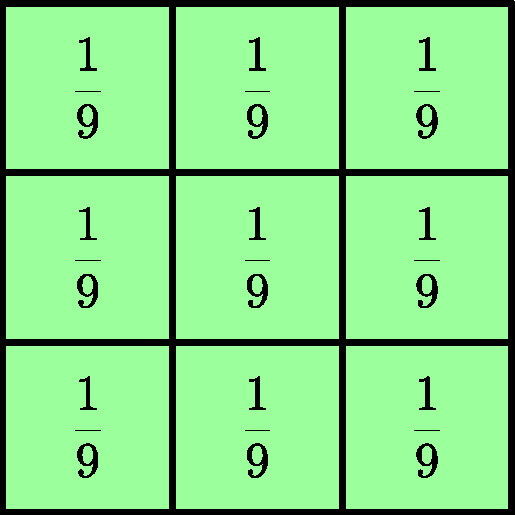
\includegraphics[height=2cm]{figs/maxmixed.pdf}
    %\caption{Maximally mixed state $\frac{1}{3}\id$}%
    }\hspace{8pt}%
    \subfigure[][]{%
    \label{fig:zero}%
    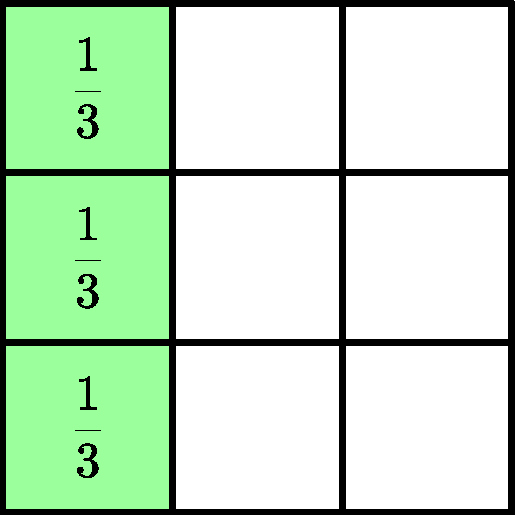
\includegraphics[height=2cm]{figs/zerostate.pdf}
    %\caption{Zero state $\ketbra{0}{0}$}%
    }\\
    \subfigure[][]{%
    \label{fig:bound}%
    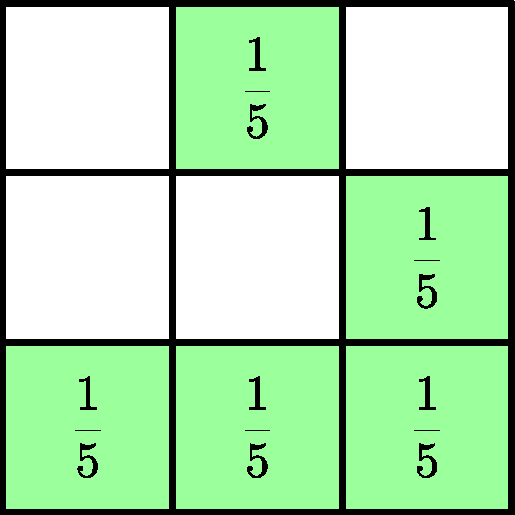
\includegraphics[height=2cm]{figs/boundstate.pdf}
    %\caption{Bound state}%
    }\hspace{8pt}%
    \subfigure[][]{%
    \label{fig:strange}%
    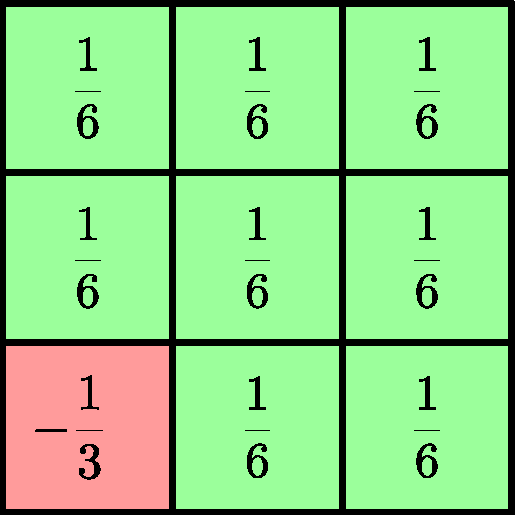
\includegraphics[height=2cm]{figs/strangestate.pdf}
    %\caption{Strange state $\ketbra{S}{S}$}%
    }
    \caption{\textbf{Qutrit Wigner distributions of varying magic.} 
    \subref{fig:maxmix} Maximally mixed state $\frac{1}{3}\id$; \subref{fig:zero} Stabilizer zero state $\ketbra{0}{0}$; \subref{fig:bound} A non-stabilizer Wigner-positive state; \subref{fig:strange} Magic strange state $\ket{{\rm{S}}} = \frac{1}{\sqrt{2}}(\ket{1} - \ket{2})$ \nick{CITE}.
    \nick{Explain what a magic state is in intro}
    }%
    \label{fig:wstate_examples}
\end{figure}

We can exploit the channel-state duality and use the normalised Choi-Jamio\l{}kowski state 
\begin{equation}\label{eq:cj}
    \frac{1}{d_A}\J(\E) \coloneqq \frac{1}{d_A}(\id \otimes \E) \sum_{i,j} \ket{ii}\bra{jj}
\end{equation}
to extend the definition of the Wigner distribution to quantum $\cptp$ operations $\E: \cal{B}(\hd[d_A]) \mapsto \cal{B}(\hd[d_B])$, 
\begin{align}\label{eq:woperation}
    \W[\bmy|\bmx]{\E} 
    &\coloneqq d_A^2 \W[\bm{\bar x} \oplus \bmy]{\frac{1}{d_A}\J(\E)} \\
    &= \frac{1}{d_B} \tr_B[A_{\bmy} \E(A_{\bmx})],
\end{align}
where $\bm{\bar x} \coloneqq (x_0, -x_1)$.

The specific form of~\cref{eq:woperation} is chosen so that Wigner distributions of operations act as transition matrices for Wigner distributions of states, $\W{\E(\rho)} = \W{\E}\W{\rho}$.
In particular, $\cptp$ operations that map between density operators of equal dimensions and have non-negative Wigner distributions correspond to stochastic matrices, as shown in~\cref{app:wigner}

The single-qudit Hadamard gate $H$ and phase gate $S$ generate the $d$-dimensional Clifford group $\cd$. \nick{CITE}
Their Wigner distributions are given by permutation matrices,
\begin{align}
    H &\coloneqq \frac{1}{\sqrt{d}}\sum_{j,k} \omega^{jk} \ketbra{j}{k}, \W[\bmy|\bmx]{H} = \delta_{y_0, -x_1}\delta_{y_1, x_0};\label{eq:H}\\
    S &\coloneqq \sum_k \tau^{k(k+1)} \ketbra{k}{k}, \W[\bmy|\bmx]{S} = \delta_{y_0, x_0}\delta_{y_1, x_0 + x_1 + 2^{-1}}.\label{eq:S}
\end{align}

%%%%%%%%%%%%%%%%%%%%%%%%%%%%%%%%%%%%%%%%

\section{Stochastic structure of magic theories}
\label{sec:struc}

\subsection{Magic fragments}\label{sec:magfrag}

Equipped with the definitions of the Wigner distribution in odd prime dimensions, we can formally recast the maximal magic theory $\Rmax$ into a stochasticity setting.
The free states correspond to proper probability distributions 
\begin{equation}
    \Fmax \coloneqq \{ \rho: \W[\bmz]{\rho} \geq 0 \text{ for all } \bmz \in \pd\}
\end{equation}

The free operations should send the set of free states $\Fmax$ into itself and completely preserve the non-negativity of the states, in the sense that $\E \in \Omax$ iff $(\id_d \otimes \E ) \sigma \in \stab$ for all odd prime dimensions $d$ whenever $\sigma \in \Fmax$.
It is shown by Wang \textit{et al.}~\cite{cit:wang} that $\Omax$ coincides with the set of operations $\E$ that correspond to stochastic Wigner distributions, 
\begin{equation}
    \Omax = \{ \E: \W[\bmy|\bmx]{\E} \geq 0 \text{ for all } \bmx, \bmy \in \pd\}.
\end{equation}

Any magic theory $\R = (\F, \O)$ is a subtheory of $\Rmax$ as explained in~\cref{sec:intro}, and as such it falls under this new stochasticity setting. 
For technical simplicity in what follows we assume that $\F$ is a closed set, and note that $\F_{\rm{ max}}$ is itself a closed set, since it is specified by a finite set of linear constraints of the form $\tr[ L\rho] \geq 0$ with operators $L \in \cal{B}(\cal{H})$ ensuring that the state is positive and Wigner-positive.


Given this context we now define the following key notion, that is central to our analysis.
\begin{definition}[\textbf{$\boldsymbol\sigma$-fragment}]\label{def:sigmafrag}
   Given a resource theory of magic $\R = (\F, \O)$, the \emph{$\sigma$--fragment of $\R$} is the resource theory $\R_\sigma = (\F, \O_\sigma)$, where the free operations are restricted to the ones that leave $\sigma$ invariant, namely
    \begin{equation}
        \O_\sigma \coloneqq \{ \E \in \O: \E(\sigma) = \sigma \}.
    \end{equation}
\end{definition}

With this basic notion defined, we now show that any resource theory of magic can be faithfully subdivided into $\sigma$--fragments, in such a way that any problem of interconversion in the parent magic theory $\R$ can be analysed across the different fragments.

\begin{theorem}
    Let $\R = (\F, \O)$ be a theory of magic.
    Every operation in $\O$ leaves at least one free state invariant,
  \begin{equation}
\O = \bigcup\limits_{\sigma \in \F} \O_\sigma.
\end{equation}
Therefore, $\rho \longrightarrow \tau$ in $\R$ if and only if $\rho \longrightarrow \tau$ in a $\sigma$--fragment of $\R$.
\end{theorem}
\begin{proof}
    Suppose $\E$ is in a $\sigma$--fragment $\O_\sigma$.
    Then it is also in $\O$, hence $\bigcup\limits_{\sigma \in \F} \O_\sigma \subseteq \O$. 
    
    Conversely, suppose $\E$ is in $\O$. 
    The free states are a closed set that is mapped one-to-one to a closed subset $\cal{S}$ of the $(d^2 - 1)$-dimensional probability simplex.
    $\cal{S}$ is convex, since any combination of free states is also free and the Wigner distribution is linear.
    Therefore, $\cal{S}$ is convex and compact as a closed convex subset of the bounded compact probability simplex.
    
    We can now view $\W{\E}$ as a stochastic, continuous mapping from $\cal{S}$ to itself, thus Brouwer's fixed point theorem \nick{CITE} implies that there exists a probability distribution $d_{\bmz}$ for some $ \bmz \in \pd$ that is a fixed point of $\W{\E}$.
    This corresponds to a free state $\sigma \coloneqq \sum_{\bmz \in \pd} d_{\bmz} A_{\bmz} \in \F$. 
    Therefore $\E \in \O_\sigma$, and so $\O = \bigcup\limits_{\sigma \in \F} \O_\sigma$. 
    
    The state interconversion result follows immediately.
\end{proof}

The zoo of all magic operation classes is summarised in ~\cref{fig:zoo}.
Completely positive-Wigner-preserving operations~\cite{cit:wang} form the operation class $\Omax$.
Therefore, $\sigma$--fragments cover this theory of magic exactly and any magic subtheory is contained within this cover.
In particular, the stabilizer operations $\so$ are contained within $\Omax$.
\begin{figure}[t]
    \centering
        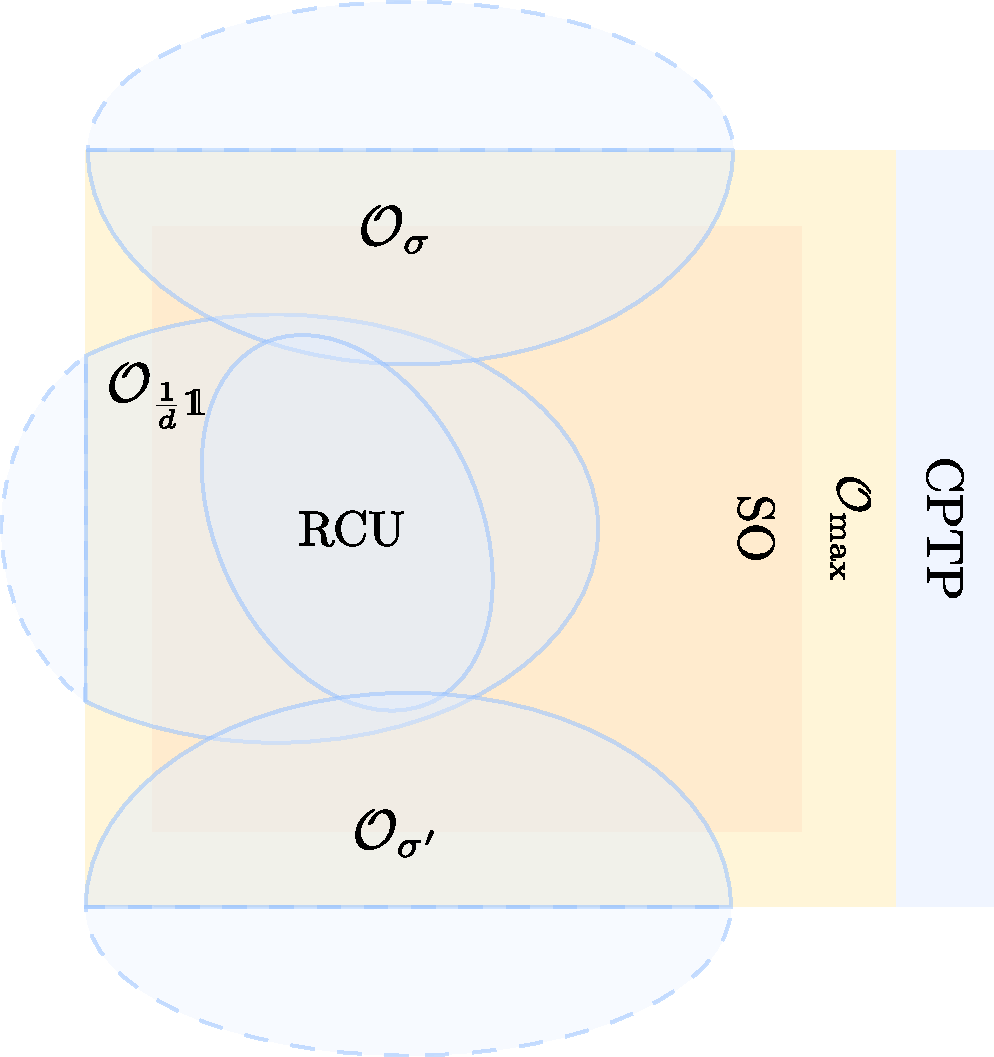
\includegraphics[scale=0.47
        ]{figs/operations.pdf}
    \caption{\textbf{Decomposition of a magic theory $\R$ intro $\sigma$--fragments.} 
	Examples of magic theories ($\so$: Stabilizer operations, $\Omax$: Completely positive-Wigner-preserving operations, $\rcu$: Random Clifford Unitaries -- subclass of $\so$) involve operations denoted by the two yellow regions, with every other established magic theory  between them.
    We introduce $\sigma$--fragments $\O_\sigma$ defined for all free states $\sigma$ that cover $\Omax$. 
    Each $\O_\sigma$ is extensible to a set of stochastic maps outside the $\cptp$ operations.
    Within each $\sigma$--fragment $\bmd$-majorization can be used allowing for an intricate, but tractable approach towards the study of magic state interconversion.
    }
    \label{fig:zoo}
\end{figure}

The subdivision of magic theories into $\sigma$--fragments is powerful because the pre-order $\prec_{\R_\sigma}$ of every $\sigma$--fragment is described by well-behaved majorization tools, as we establish in~\cref{sec:major}.

\subsection{Majorization of quasi-probabilities in $\sigma$--fragments}\label{sec:major}

Majorization is a collection of powerful tools that has recently found many applications in quantum information theory \nick{CITE}.
It can describes the \nick{disorder / non-uniformity} of distributions that undergo stochastic transformations.

To formally state majorization results, we first denote by $\stoch$ the set of $(d \times d)$ stochastic matrices that preserve the probability vector $\bmd$. \nick{Should we introduce notation directly in the magic setting?}
Specifically, for any $S \in \stoch$, all matrix elements are non-negative, all rows sum to $1$ and $S\bmd = \bmd$.
\iffalse
\begin{enumerate}
    \item $S_{ij} \geq 0$ for all $i, j \in \zd$;
    \item $\sum\limits_{j=1}^n S_{ij} = 1$ for all $i \in \zd$;
    \item $S\bmd = \bmd$.
\end{enumerate}
\fi
The set $\stoch$ forms a group under matrix multiplication for all $\bmd$ with positive components.

Majorization finds an important application on quantum thermodynamics in the absence of coherence.
The use of majorization in this setting provides useful intuition for our purposes.
At any given temperature $\beta$, the thermal state $\gamma_\beta$ is thermodynamically the most disordered state. 
Thermal operations are defined as operations that cannot extract energy from the Gibbs state, $\E(\gamma_\beta) = \gamma_\beta$.
Convertibility between states via thermal operations is equivalent to a stochasticity condition on the energy level populations of the states \nick{CITE}.
Roughly, the statement is that there exists a thermal operation $\E$ such that $\tau = \E(\rho)$ if and only if there exists a a matrix $S \in \stoch$ such that $\bm{q} = S\bm{p}$, where $\bm{q}, \bm{p}$ and $\bmd$ and the energy level population vectors of $\tau, \rho, \gamma_\beta$ respectively.

Drawing intuition from this setting, we can define majorization as follows.
\begin{definition}[\textbf{$\boldsymbol\bmd$-majorization}]\label{def:dmajor}
    Given $\bmx, \bmy, \bmd \in \reals^d$, such that the components of $\bmd$ are positive, $\bmy$ is said to $\bmd$-majorize $\bmx$, iff there exists a matrix $S \in \stoch$ such that $\bmx = S\bmy$.
\end{definition}
We denote this pre-order by $\bmx \prec_{\bmd} \bmy$.
If $\bmd = \frac{1}{d}\bm{1}$, the $d$-dimensional uniform distribution, then $\stoch$ is the set of doubly stochastic matrices and we retrieve the familiar notion of majorization in entanglement theory. \nick{CITE}

The pre-order $\prec_{\R_\sigma}$ of the $\sigma$--fragment $\R_\sigma = (\F, \O_\sigma)$ between $d$-dimensional states corresponds to the majorization pre-order $\prec_{\W{\sigma}}$ between their $d^2$-dimensional Wigner distributions.
For simplicity we shall merge the notation into $\prec_\sigma$, as there is little risk of confusion.


\begin{theorem}\label{thm:sigmamajor}
    Let $\R = (\F, \O)$ be a theory of magic. Then $\rho \longrightarrow \tau$ is possible \nick{only if}  $\W{\tau} \prec_\sigma \W{\rho}$ within a $\sigma$--fragment.
\end{theorem}
\begin{proof}
Suppose we can convert $\rho$ into $\tau$ in the magic theory. 
Thus there is some $\O_\sigma$ and some $\E \in \O_\sigma$ such that $\E(\rho) = \tau$, and $\E(\sigma)=\sigma$. 
Therefore, the Wigner distribution of this free operation satisfies $\W{\E} \in \stochw$ and $\W{\E}\W{\rho} = \W{\tau}$. 
Since $\sigma$ is \nick{full-rank} and free, its Wigner distribution is strictly positive in all components, so it directly follows from~\cref{def:dmajor} that $\W{\tau} \prec_{\sigma} \W{\rho}$.
\end{proof}
This result can be understood as an extension of the idea of a magic monotone, where we replace $\M(\tau) \leq \M(\rho)$ with $\W{\tau} \prec_\sigma \W{\rho}$. 
However the majorization constraints can be used to place upper bounds on magic state distillation in a way that allows one to incorporate the physics of the allowed operations -- this enables us to bound how much magic can be distilled via quantum operations that, for example, preserve the equilibrium state of the system, or via operations that are symmetric about the $Z$-axis of the Bloch sphere.

This approach can also provide \emph{lower bounds} on distillation, however now more structure about the specific free operations must be included. 
\nick{This is more involved and we discuss this later in the paper.
Also mention relative majorization somewhere}

\subsection{Majorization computations in $\sigma$--fragments}
A numerically efficient reformulation of $\bmd$-majorization is provided by Lorenz curves.
Let the vector $\bmu^\downarrow$ denote the vector $\bmu \in \reals^d$ with its components arranged in non-increasing order.
\begin{definition}[\textbf{Lorenz curve}]\label{def:lc}
    Let $\bmz, \bmd \in \reals^d$, where the components of $\bmd$ are positive with $D = \sum_{i=1}^d d_i$ and denote by $\tilde{\bmz} \coloneqq (z_1/d_1, \dots, z_d/d_d)^T$ the vector of ratios between the corresponding components of $\bmz$ and $\bmd$.
    
    Finally, denote by $\pi: \zd \mapsto \zd$ the permutation that sorts $\tilde{\bmz}$, $(\tilde{\bmz}^\downarrow)_i = z_{\pi(i)}$ for all $i=1,\dots,d$.
    
    Consider the piecewise linear curve obtained by joining the points $\{(0,0)\} \cup \{ (x_k, \lc{\bmz}{\bmd}(k)) \}_{k=1,\dots,d}$, where
    \begin{equation}\label{eq:lorenz}
        (x_k, \lc{\bmz}{\bmd}(k)) \coloneqq \left( \frac{1}{D}\sum_{i=1}^k d_{\pi(i)}, \sum_{i=1}^k z_{\pi(i)} \right) \in \mathbb{R}^2.
    \end{equation}
    We define the set of points on this curve, $\lc{\bmz}{\bmd}(x),\ x \in [0,1]$, as the \emph{Lorenz curve} of vector $\bmz$ with respect to $\bmd$.
\end{definition}
Components $x_k$ are rescaled by $D$ so that comparison of curves with unequal dimensions is possible.
In fact, the Lorenz curves $\lc{\bmz}{\bmd}$ and $\lc{\bmz \otimes \bmd}{\bmd \otimes \bmd}$, where $\otimes$ denotes the Kronecker product, are identical.
Furthermore, a Lorenz curve $\lc{\bmz}{\bmd}(x)$ is always concave in $x$, since it consists of $d$ line segments each with slope $(\tilde{\bmz}^\downarrow)_i$ for $i=1,\dots,d$ which is non-increasing by definition.
Finally, points on the interior of the Lorenz curve connecting line segments of different slopes are called \emph{elbows}.

A vector $\bmy$ \emph{$\bmd$--majorizes} another vector $\bmx$ if and only if the Lorenz curve $\lc{\bmy}{\bmd}$ lies above Lorenz curve $\lc{\bmx}{\bmd}$, thus reducing $\bmd$--majorization into a finite set of inequalities.
\begin{theorem}\label{thm:dmajor}
    Let $\bmx, \bmy, \bmd \in \reals^d$, such that the components of $\bmd$ are positive. 
    Then, $\bmx \prec_{\bmd} \bmy$ if and only if $\lc{\bmx}{\bmd}(x) \leq \lc{\bmy}{\bmd}(x)$ for all $x \in [0,1]$ with strict equality at $x=1$.
\end{theorem}
A restatement of the theorem including more equivalent conditions and a proof are provided in~\cref{app:major}.
An example of comparison between different Lorenz curves is illustrated in~\cref{fig:lctoy}.
\begin{figure}
    \centering
    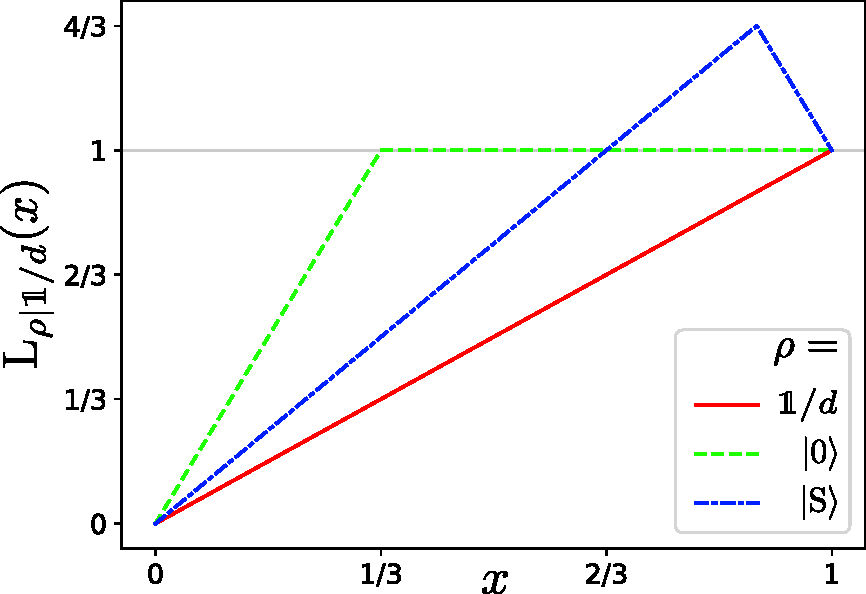
\includegraphics[height=5cm]{figs/lctoy.pdf}
    \caption{Example of different Lorenz curves for quasi-probability vectors under $\bmd$-majorization.
    Vectors $\bmy$ and $\bmd$ are simply probability distributions.
    The curve corresponding to vector $\bmd$ is always the line segment connecting $(0,0)$ and $(1,1)$, so that any other Lorenz curve lies above it, for example $\bmx \prec_{\bmd} \bmd$.
    Curves $L_k(\bmx|\bmd)$ and $L_k(\bmy|\bmd)$ intersect, so $\bmx \nprec_{\bmd} \bmy$ as well as $\bmy \nprec_{\bmd} \bmx$.
    \nick{Recast in terms of magic - replace with~\cref{fig:test}?}
    }
    \label{fig:lctoy}
\end{figure}

It is now straightforward to construct Lorenz curves for Wigner distributions in any $\sigma$--fragment.
As we have seen in~\cref{thm:sigmamajor}, for any full-rank free state $\sigma$ we have that $\W{\sigma}$ is a strictly positive full-rank probability distribution, and so one can define a corresponding notion of $d$--majorization on \emph{quasi}--distributions.
We write $\lc{\rho}{\sigma}(x)$ for the Lorenz curve of $\W{\rho}$ with respect to $\W{\sigma}$.

We now establish important properties of Lorenz curves that are independent of the $\sigma$--fragment they are defined in.
\begin{proposition}\label{thm:lccont}
	The Lorenz curve $\lc{\rho}{\sigma}(x)$ of a state $\rho$ with respect to state $\sigma$ is uniformly continuous in $\sigma$. 
	\nick{In the sense that if $\sigma$ and $\sigma'$ are $\delta$-close with respect to a state norm, then the curves $\lc{\rho}{\sigma}(x)$ and $\lc{\rho}{\sigma'}(x)$ are $\epsilon$-close at all $x \in [0,1]$.
	I think this clears up the narrative quite a bit? - Should we keep and prove this result?} \ddd{[Is a nice result...hmm let's wait and see. It might distract from the main message.]}
\end{proposition}
The proof of this important result is in \nick{the appendix}.
The consequence of this statement is that infinitesimal changes in state $\sigma$ only result in infinitesimal shifts of the $\sigma$--fragment.
Therefore, Lorenz curves and majorization analysis in general \nick{behave nicely in the presence of / are robust under} imperfections in the experimental implementation of quantum operations.
In particular, any $\sigma_0$--fragment defined by a non full-rank state $\sigma_0$ can be approximated by a $\sigma$--fragment defined by a full-rank $\sigma$ which is arbitrarily close to $\sigma_0$, such that $\sigma = (1-\epsilon)\sigma_0 + \epsilon\frac{1}{d}\id$, for some small $\epsilon > 0$.
Such $\sigma_0$--fragments may include important stabilizer operations such that the replacement channel defined as $\E(\rho) = \sigma_0$ for all states $\rho$.
For simplicity, we restrict analysis to $\sigma$-fragments, where $\sigma$ is full-rank.

Normalisation of the Wigner distribution \nick{REF} ensures that for all quantum states $\rho$, $\lc{\rho}{\sigma}(x) \geq 0$ and $\lc{\rho}{\sigma}(1) = 1$.
As a consequence, checking whether a state conversion $\rho \longrightarrow \tau$ is possible as per~\cref{thm:dmajor}, reduces to the condition $\lc{\rho}{\sigma}(x) \leq \lc{\tau}{\sigma}(x)$ for all $x \in [0,1]$.
We stress that $0 \leq \lc{\rho}{\sigma}(x) \leq 1$ for all $x \in [0,1]$ if and only if $\rho$ is a positive Wigner state.

The area $\A_\sigma(\rho)$ between the curve $L_{\rho|\sigma}$ and the line $y=1$ is a resource monotone in the $\sigma$--fragment. 
This is clear because for any state conversion $\rho \longrightarrow \tau$ for some $\E \in \O_\sigma$, the Lorenz curve $L_{\tau|\sigma}$ is lower than $L_{\rho|\sigma}$, hence $\A_\sigma(\E(\rho)) \leq \A_\sigma(\rho)$.
The exact form of the monotone is given in~\cref{app:areamono}

\ddd{[relate to mana?]} \nick{the area depends on several positive Wigner components and cannot be written as a function of mana annoyingly - should we include the area? Have a look at~\cref{app:areamono}}

%%%%%%%%%%%%%%%%%%%%%%%%%%%%%%%%%%%%%%%%%

\section{Magic state interconversion and Lorenz curve comparison}
\label{sec:distill}

Any quantum circuit aiming at a given magic state conversion $\rho \longrightarrow \tau$ possesses certain symmetries according to~\cref{thm:frag} that allow us to study the conversion within only certain $\sigma$-fragments.
As a simple example, the dephasing channel
\begin{equation}\label{eq:dephase}
	\Delta(\rho) = \sum_{k \in \zd} \ketbra{k}{k}\rho\ketbra{k}{k}
\end{equation}
removes coherent phases in the computational basis and therefore leaves exactly all mixtures of computational basis states invariant.
A model circuit consisting only of such dephasing channels can be fully analysed in the $\sigma$--fragments for the pure computational basis states $\sigma$ \nick{as seen in a theorem in the appendix}.

Lorenz curves provide an efficient method of numerically checking if a certain state conversion is impossible within a $\sigma$--fragment by exploiting the equivalence with $d$--majorization stated in~\cref{thm:dmajor}.
Such methods are often more conclusive than magic monotones as we discuss in section~\cref{sec:scmana}.

\subsection{Majorization in magic theories}\label{sec:scmana}
We now discuss majorization features common to all fragments, before specialising to particular $\sigma$--fragments and how analysis in them proceeds.

As discussed above, we know that every magic interconversion problem can be analysed across all $\sigma$--fragments that reflect symmetries of the circuit and moreover the pre-order in each such fragment is exactly specified by $d$--majorization.

Consider a general magic state interconversion in $\O_\sigma$, 
\begin{equation}
	\rho \xrightarrow{\E \in \O_\sigma} \tau.
\end{equation}

Magic theories utilise monotone bounds of the form
\begin{equation}\label{eq:majbound}
    \M(\rho) \geq \M(\tau),
\end{equation}
to determine whether the interconversion is allowed.
Monotone bounds hold independently of $\sigma$--fragments, therefore they provide no understanding with regard to the type of operations that allow the interconversion.

New bounds can be obtained in the $\sigma$--fragment by pointwise Lorenz curve comparison of the initial and target states,
\begin{equation}\label{eq:majbound}
    \lc{\rho}{\sigma}(x) \geq \lc{\tau}{\sigma}(x),\ x\in [0,1].
\end{equation}
This inequality is parametrised by $x$ and if it is not satisfied at any point $x$, then the Lorenz curves intersect and the conversion is impossible.
We can refine the independent constraints stemming from this inequality and consider it at only the locations of the target state elbows.
\begin{theorem}\label{thm:elbows}
	Let $\rho, \tau$ be two quantum states with Lorenz curves $\lc{\rho}{\sigma}(x), \lc{\tau}{\sigma}(x)$ in the $\sigma$-fragment.
	
	Let $\tt$ be the number of elbows of $\lc{\tau}{\sigma}(x)$ and $E \coloneqq \{x_1, \dots, x_\tt\}$ be their locations.
	
	Then, $\lc{\rho}{\sigma}(x) \geq \lc{\tau}{\sigma}(x)$ for all $x \in [0,1]$ iff $\lc{\rho}{\sigma}(x_{\ii}) \geq \lc{\tau}{\sigma}(x_{\ii})$ for all $\ii =1,\dots,\tt$.
\end{theorem}
A proof is provided in~\cref{app:lc_constraints}.
Any of the $t$ inequalities in the theorem provides a valid contraint leading to some upper distillation bound, and the more one cosiders, the stricter the bound is.

\nick{We can skip mana and just discuss sum-negativity}

One of the most fundamental and commonly used magic monotones is the \emph{mana} of a state \nick{CITE}, defined as
\begin{equation}
    \mana{\rho} \coloneqq \log{(2\sn{\rho}+1)},
\end{equation}
where the \emph{sum-negativity} ($\rm{sn}$) \nick{CITE} is the sum of the negative components in $\W{\rho}$,
\begin{equation}
    \sn{\rho} \coloneqq \sum\limits_{\bmx: \W[\bmx]{\rho} < 0} \abs{\W[\bmx]{\rho}}.
\end{equation}
Mana is an additive\footnote{It satisfies the condition $\mana{\rho_1 \otimes \rho_2} = \mana{\rho_1} + \mana{\rho_2}$ which is practical is distillation settings.} magic monotone, so it provides a necessary condition for magic state interconvertibility.

Here, we show that its properties can be viewed as majorization-based, and independent of the particular $\sigma$--fragment one works in.
In fact, our current setting makes it apparent that the mana provides a weaker condition than majorization for all magic state interconversions.

We first show that the Lorenz curve maximum of state $\rho$ is independent of the $\sigma$--fragment and directly related to its sum-negativity.
\begin{lemma}\label{lem:lcmax}
	Given a quantum state $\rho$, the maximum of its Lorenz curve $\lc{\rho}{\sigma}$ is independent of the $\sigma$--fragment in which it is defined and equal to $1+\sn{\rho}$.
\end{lemma}
\begin{proof}
	For notational simplicity, denote $(\W{\rho})_i = \W[\bmx]{\rho},\ i = 1,\dots, d^2$ and similarly for $\W{\sigma}$.
	We choose the index mapping so that the vector of component ratios, 
	\begin{equation}
		\tilde{\bm{w}} \coloneqq \left(\frac{(\W{\rho})_1}{(\W{\sigma})_1}, \dots, \frac{(\W{\rho})_{d^2}}{(\W{\sigma})_{d^2}} \right)^T,
	\end{equation}
	is sorted in the sense that $\tilde{\bm{w}} = \tilde{\bm{w}}^\downarrow$.
	Note that all components of $\W{\sigma}$ are positive, so $(\tilde{\bm{w}})_i \geq 0$ if and only if $(\W{\rho})_i \geq 0$ for any $i=1,\dots,d^2$.
	
	Let $\ii_\star$ be the index of the smallest non-negative component of $\tilde{\bm{w}}^\downarrow$.
	Then, $(\W{\rho})_i < 0$ if and only if $i > \ii_\star$, so the maximum of Lorenz curve $\lc{\rho}{\sigma}(x)$ takes the value 
	\begin{equation}
		\lc{\rho}{\sigma}(x_{\ii_\star}) = \sum_{i=1}^{\ii_\star} (\W{\rho})_i,
	\end{equation}
	and is achieved at
	\begin{equation}\label{eq:maxloc}
		x_{\ii_\star} \coloneqq \sum_{i=1}^{\ii_\star} (\W{\sigma})_i.
	\end{equation}

	The location of the maximum ($x=x_{\ii_\star}$) varies from fragment to fragment, but its value is independent of $\sigma$,
	\begin{equation}
		\lc{\rho}{\sigma}(x_{\ii_\star})
		= \sum\limits_{\bmx: \W[\bmx]{\rho} \geq 0} \W[\bmx]{\rho}
		= 1 + \sn{\rho}.
	\end{equation}
	
\end{proof}

We can therefore view mana as just one feature of the Lorenz curve, namely its maximum value. 
This implies the following result.
\begin{theorem}\label{thm:bounds}
    Given a magic state conversion $\rho \longrightarrow \tau$, the majorization condition is stronger than the mana condition in every $\sigma$--fragment.
\end{theorem}
\begin{proof}
    The maximum of the Lorenz curve of a state $\rho$ is independent of the $\sigma$--fragment due to~\cref{lem:lcmax}, and can be expressed as an increasing function of mana,
    \begin{equation}
        \max_{x\in[0,1]}{\lc{\rho}{\sigma}(x)} = 1 + \sn{\rho} = \frac{1}{2} \left( 1 + e^\mana{\rho} \right).
    \end{equation}
    Therefore, the majorization bound
    \begin{equation}
    	\lc{\rho}{\sigma}(x) \geq \lc{\tau}{\sigma}(x),\ x\in[0,1]
    \end{equation}
    implies the order $\max_{x\in[0,1]}{\lc{\rho}{\sigma}(x)} \geq \max_{x\in[0,1]}{\lc{\tau}{\sigma}(x)}$, equivalent to the mana condition $\mana{\rho} \geq \mana{\tau}$.
\end{proof}

Denote an $n$-copy, $\epsilon$-noisy magic state $\rho$ in the $\sigma$--fragment by
\begin{equation}\label{eq:dist}
    \rho(\epsilon)\too{\nn} = \left[ (1 - \epsilon) \rho + \epsilon \sigma \right]\too{\nn},
\end{equation}
and consider the general magic state distillation (MSD) / purification process
\begin{equation}
		\rho(\epsilon)\too{\nn} \xrightarrow{\E \in \O_\sigma} \rho(\epsilon')\too{\tt},
\end{equation}
where it is converted into a $\tt$-copy, $\epsilon'$-noisy state, such that the number of copies has decreased ($\tt < \nn$), but the state is less noisy ($\epsilon' < \epsilon$).

The more noisy the initial state is, the more copies needed to reach the target. 
We make this idea precise by defining the \emph{noise level threshold} as
\begin{equation}\label{eq:ethresh}
	\begin{split}
	\epsilon_{\rm{th}}(\nn, \tt, \epsilon', \sigma) \coloneqq &\sup{\{\epsilon:\ \lc{\rho(\epsilon)\too{\nn}}{\sigma}}(x) \geq \\
	&{\lc{\rho(\epsilon')\too{\tt}}{\sigma}(x),\ x\in[0,1]\}}.
	\end{split}
\end{equation}
The MSD process~(\ref{eq:dist}) is impossible for all $\epsilon > \epsilon_{\rm{th}}(\nn, \tt, \epsilon', \sigma)$.

\nick{Can also define a distillation bound
\begin{equation}\label{eq:ethresh}
	\nn_{\rm{th}}(\epsilon, \epsilon', \sigma) \coloneqq \min{\{\nn: \lc{\noisysn}{\sigma} \geq \lc{\noisys(\epsilon')}{\sigma}\}}.
\end{equation}}

In general, the Wigner components of an $\NN$-copy state $\rho\too{\NN}$ can be calculated directly from $\W{\rho}$ by convolution of the distribution with itself,
\begin{equation}
	\W{\rho\too{\NN}} = \rm{W}_{\rho}\too{\NN},
\end{equation}
where $\otimes$ can be interpreted as the usual Kroenecker product in the last expression.
Furthermore, single-copy Lorenz curves are simply additive in noise, 
\begin{equation}
\lc{(1-\epsilon)\rho + \epsilon\sigma}{\sigma} = (1-\epsilon)\lc{\rho}{\sigma} + \epsilon\lc{\sigma}{\sigma},
\end{equation}
for any $\sigma, \rho$.
This is not true for higher number of copies.

An important example is the purificiation process~\cref{eq:dist} of the qutrit Strange state $\ketbra{\rm{S}}$,
\begin{equation}
    \noisys(\epsilon) = (1 - \epsilon) \ket{\rm{S}}\bra{\rm{S}} + \epsilon \sigma,
\end{equation}
in $\O_\sigma$, where $\ket{\rm{S}}$ is defined in~\cref{fig:strange}. 
For $\epsilon=0$, this state is a qutrit of maximal sum-negativity \nick{CITE} and therefore acts as the ideal distiallation target, analogous to a Bell state in bipartite entangelement theory.

In~\cref{fig:lcs}, we illustrate the Lorenz curves of pure and noisy $n$-copy Strange states for $n$ up to $4$ in different $\sigma$-fragments.
\begin{figure}%
    \centering
    \subfigure[][]{%
    \label{fig:lcs_maxmix}%
    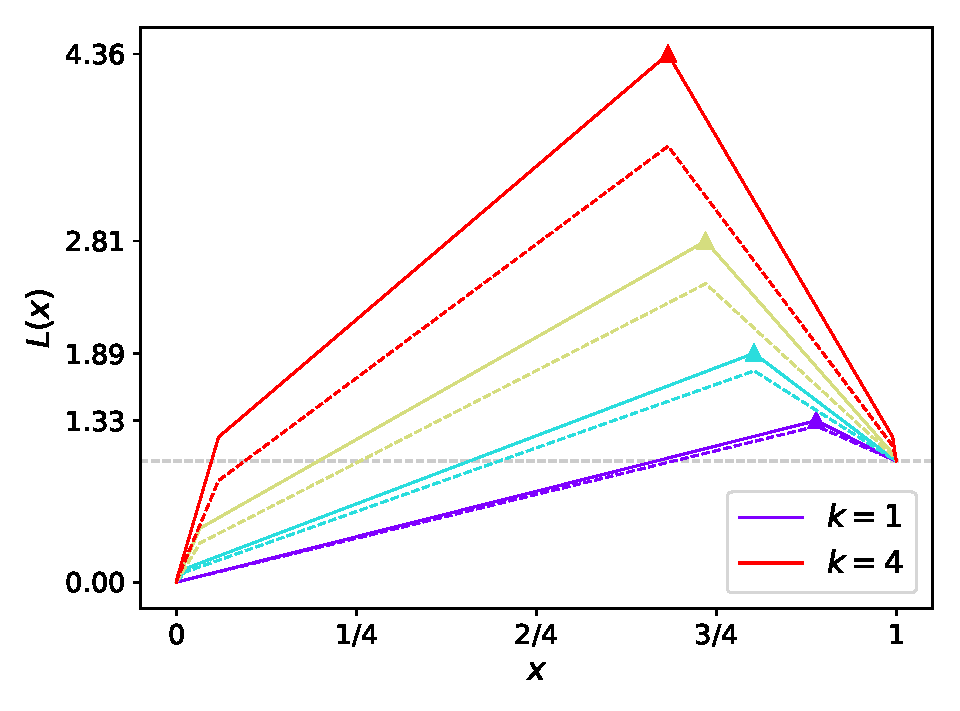
\includegraphics[height=3cm]{figs/lcs_maxmix.pdf}
    %\caption{Maximally mixed state $\frac{1}{3}\id$}%
    }\hspace{1pt}%
    \subfigure[][]{%
    \label{fig:lcs_thermal}%
    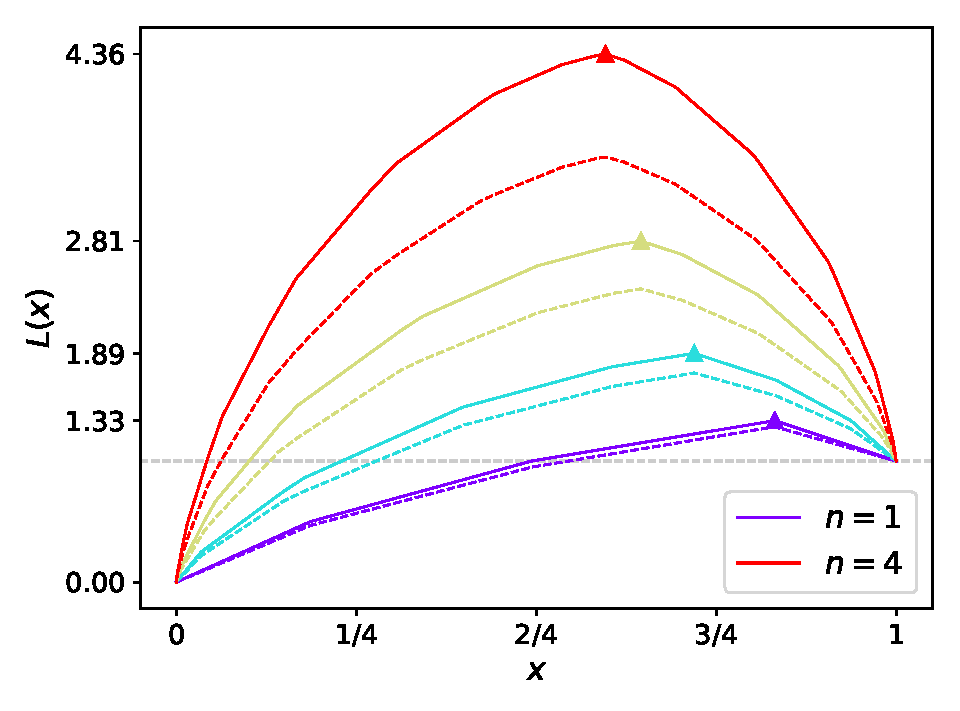
\includegraphics[height=3cm]{figs/lcs_thermal.pdf}
    %\caption{Zero state $\ketbra{0}{0}$}%
    }\\
    \subfigure[][]{%
    \label{fig:lcs_zero}%
    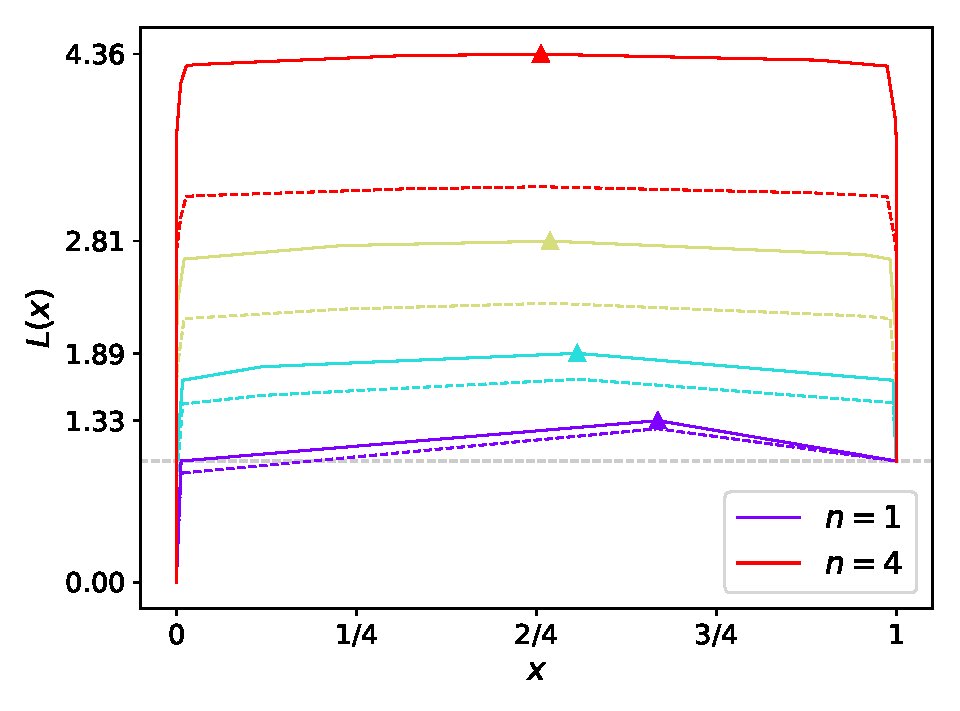
\includegraphics[height=3cm]{figs/lcs_zero.pdf}
    %\caption{Bound state}%
    }\hspace{1pt}%
    \subfigure[][]{%
    \label{fig:lcs_one}%
    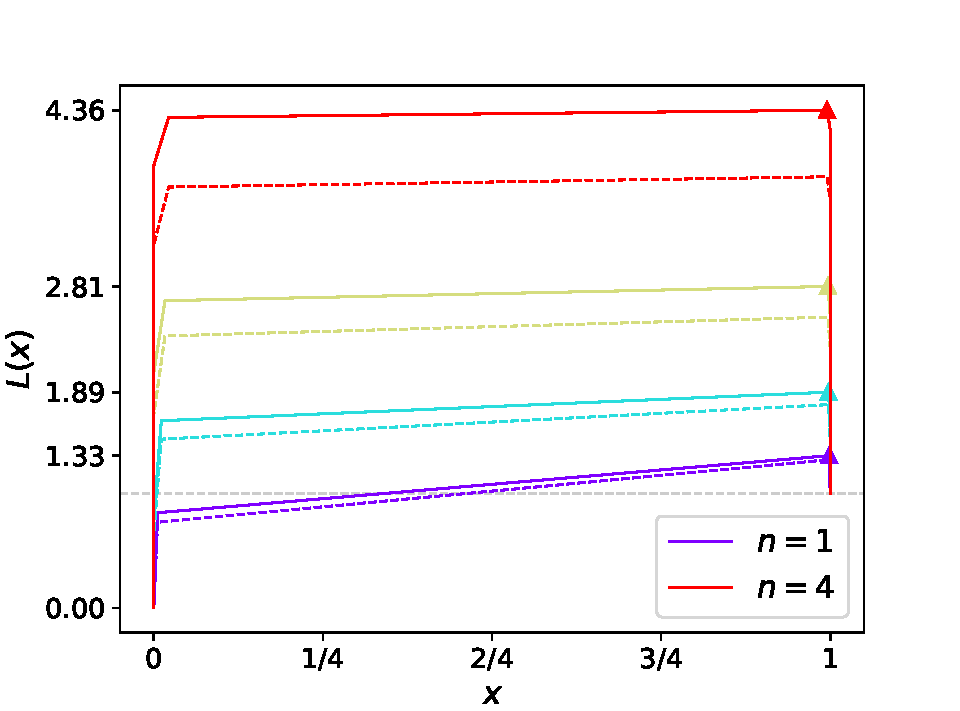
\includegraphics[height=3cm]{figs/lcs_one.pdf}
    %\caption{Strange state $\ketbra{S}{S}$}%
    }
    \caption{\textbf{Lorenz curves of Strange state copies.} Lorenz curves of $\noisysn$ for $\nn=1,2,3,4$.
    Solid lines represent pure Strange states ($\epsilon = 0$); dashed lines represent noisy Strange states ($\epsilon = 0.1$).
    \subref{fig:lcs_maxmix} Unital fragment; \subref{fig:lcs_thermal} Thermal fragment with $H = (0,1,2)$ and $\beta = 0.5$; \subref{fig:lcs_zero} Fragment $\O_{\ketbra{0}{0}}$ (corresponds to red curve in~\cref{fig:stab_distill}); \subref{fig:lcs_one} Fragment $\O_{\ketbra{1}{1}}$ (corresponds to blue curve in~\cref{fig:stab_distill}).
    The elbows of a curve are the non-differentiable points that form ``angles'' between consecutive line segments.
    }%
    \label{fig:lcs}
\end{figure}

In the following sections, we address the question of state interconversions in various $\sigma$--fragments, including concrete examples of the Strange state distillation process. \nick{adapt}

\section{Magic in unital and thermal fragments}\label{sec:unital}
The unital fragment encompasses the circuits which preserve the maximally mixed state ($\id/d$) and so it includes many important families of circuits.

MSD circuits in principle consist of bulk sequences of random Clifford unitaries ($\rcu$)\nick{CITE}, depicted in~\cref{fig:zoo}.
Operations in $\rcu$ can be expressed as
\begin{equation}
    \E(\rho) = \sum_i p_i U_i \rho U_i^\dagger,\ U_i \in \cd.
\end{equation}
Depending on the symmetries of such operations, a Clifford sequence may belong in other $\sigma$--fragments as well.
In this case, the majorization condition~(\ref{eq:majbound}) needs to be checked in all the $\sigma$-fragments that reflect the symmetries of the operation sequence.

In general, noisy circuits are well-described by the unital fragment.
To see this, consider incorporating noisy channels in the circuit, for example dephasing channels as in~\cref{eq:dephase} defined in different bases.
This process destroys the circuit symmetries, except for the invariance of the maximally mixed state.
Dephasing and bit-flip error channels are examples of the many error-inducing channels that respect the unital symmetry. \nick{expand}

In~\cref{fig:unital_distill}, we examine the Strange state distillation process of~\cref{eq:dist} with $\epsilon' = 0.05$ which describes all circuits that respect the unital symmetry.
Thresholds provided by Lorenz curve comparison are always much stricter than mana thresholds.
\nick{Explain asymptotic behaviour?}
\begin{figure}[h]
    \centering
    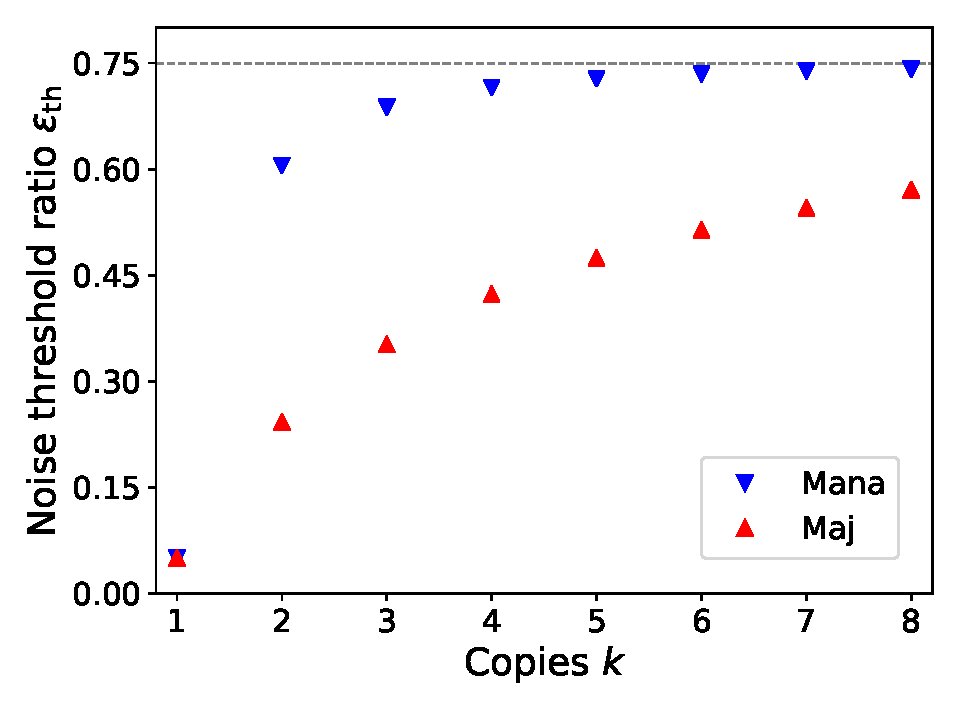
\includegraphics[scale=0.5]{figs/unital_distill.pdf}
    \caption{\textbf{Noise thresholds in unital fragment.} Mana and Lorenz curve noise thresholds for the Strange state purification process in~\cref{eq:dist} with $\epsilon' = 0.05$.
    Lorenz curve comparison consistently gives stricter bounds as proven in~\cref{thm:bounds}.
    The line $\epsilon = \frac{3}{4}$ indicates the threshold noise beyond which the Strange state no longer contains negativities. 
    \nick{Redo figure}
    }
    \label{fig:unital_distill}
\end{figure}

\iffalse
% Copies plot
\begin{figure}
    \centering
    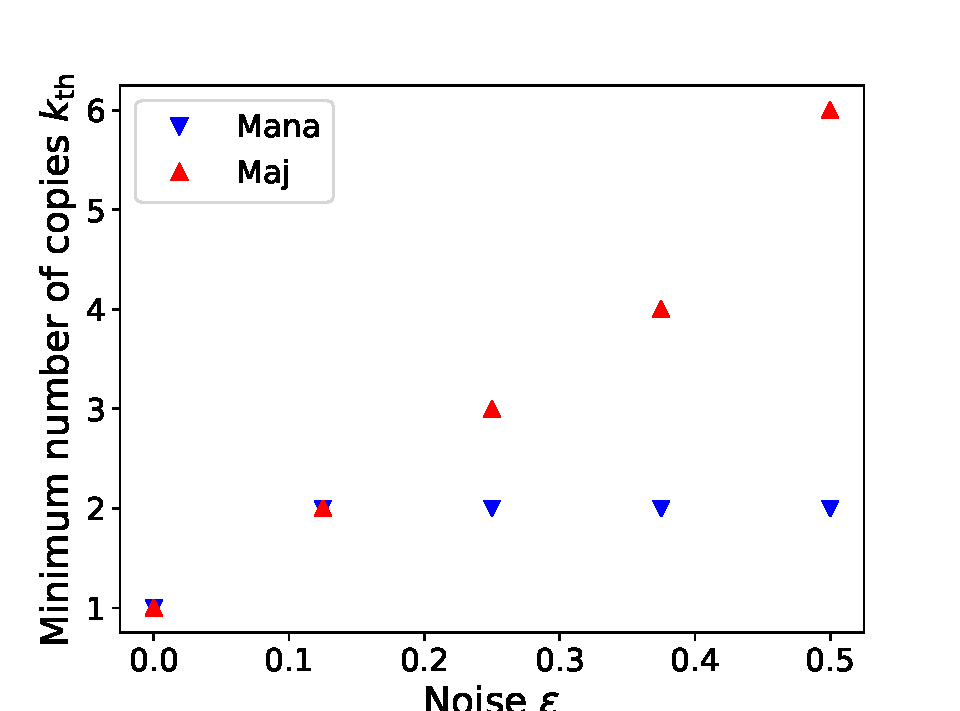
\includegraphics[scale=0.5]{figs/unital_distill_copies.pdf}
    \caption{\textbf{Copies required for Strange state distillation.} Mana and Lorenz curve copy thresholds for the Strange state purification process in~\cref{eq:sdist} with $\epsilon_\tau = 0.05$.
    Lorenz curve comparison consistently provides higher low bounds on the number of noisy Strange state copies required.
    }
    \label{fig:unital_distill_copies}
\end{figure}
\fi

\null\newpage

\subsection{Distillation rate bounds in the unital fragment}\label{sec:lcsu}

We would now like to study the constraints coming solely from majorization in the unital fragment. 
We consider the problem of purifying $\nn$ copies of a noisy strange state $\noisysn$ into a smaller number of copies $\tt$ of a less noisy strange state $\noisys(\epsilon')\too{\tt}$, with $\epsilon' \le \epsilon$ and $\tt \leq \nn$. 
Since the state $\frac{1}{3} \id$ is free, the interconversion problem is unaffected if we tensor in copies of it. More precisely the associated Lorenz curve in invariant under tensoring in arbitrary many copies of this free state.
This turns out to simplify the Lorenz curve analysis, and so we focus on the process,
\begin{equation}\label{eq:sudist}
	\noisys\too{\nn} \longrightarrow \noisys(\tt, \epsilon', \nn - \nn') \coloneqq  \noisys(\epsilon')\too{\tt} \otimes \left( \frac{1}{3}\id \right)\too{(\nn-\tt)},
\end{equation}
where all copies $\nn, \tt, \nn - \tt$ are even.
Since the initial state can be written in the form $\noisys(\nn, \epsilon, 0)$, it suffices to construct the Lorenz curve $\lc{\noisys}{\id/3}(x)$ for the generic noisy strange state $\noisys(\nn, \epsilon ,\tt)$.
This curve is defined at $9^\nn$ points between $0$ and $1$.
The exact expressions for the coordinates of these points can take $8$ different forms, depending on whether the noise level $\epsilon$ is greater than or less than $\frac{3}{7}$, the parity of the number of copies $\nn$ is even/odd and the location relative to the curve peak is on the left hand side (LHS -- including the maximum) / right hand side (RHS).
The full details are provided in~\cref{app:lcsu_technical}.

Here we focus on the case of Lorenz curves of even copies $\nn, \tt$ and low noise levels ($\epsilon \leq 3/7$).
The part of the curve on the LHS of its peak is constructed by the positive components of the state Wigner distribution that take values $w_\ii$, with associated multiplicities $\mlt_\ii$,
\begin{align}
	w_\ii &= \left( \frac{1}{6} - \frac{1}{18}\epsilon \right)^{2\ii}\left( -\frac{1}{3} + \frac{4}{9}\epsilon \right)^{\nn-2\ii}, \\
	m_\ii &= 8^{2\ii}\binom{\nn}{2\ii},
\end{align}
where $i=0,\dots,\frac{n}{2}$.
From this, it is readily seen that $\lc{\rho}{\id/3}(x)$ has elbows on the LHS of its peak located at points $x=x_\ii$, where
\begin{equation}
	x_\ii = \Phi_+ \left( 2\ii; \nn , \frac{8}{9} \right),
\end{equation}
with $\ii = 0,1, \dots , n$ and where $\Phi_+(i,n,p)$ is an even-power cumulant distribution function given by
\begin{equation}
	\Phi_+(2\ii; \nn, p) \coloneqq \sum_{\dummy=0}^{\ii} \binom{\nn}{2\dummy} p ^{2\dummy} (1-p)^{\nn-2\dummy}.
\end{equation}
We provide technical details on the function $\Phi_+$ in the appendices.

The value of the Lorenz curve at an elbow is given by
\begin{equation}
	\lc{\rho}{\id/3}(x_{\ii}) \equiv L_{\ii} =  \left( \frac{5}{3} - \frac{8}{9}\epsilon\ \right)^{\nn} \Phi_+\left(2i;\nn,\frac{12-4\epsilon}{15-8\epsilon}\right),
\end{equation}
and we define $(x_{-1}, L_{-1}) = (0,0)$.

\iffalse
The coordinates of any point on the Lorenz curve LHS can be expressed as convex sums of the neighbouring elbows,
\begin{align}
    x_{\ii\jj\kk} &= \left( 1-p_{\ii\jj\kk}\right) x_{\ii-1} + p_{\ii\jj\kk} x_{\ii} \label{eq:lcsu_xcoord}\\
    L_{\ii\jj\kk} &= \left( 1-p_{\ii\jj\kk} \right) L_{\ii-1} + p_{\ii\jj\kk} L_{\ii}, \label{eq:lcsu_lcoord}
\end{align}
where we use a three-index parametrisation for the coordinates, with $\ii$ the index of the elbow that follows, $\jj = 1,\dots,\mlt_\ii$ and $\kk=1,\dots,9^{2(\nn-\tt)}$.
Therefore, for the initial state $\noisys\too{2\nn}$ we have
\begin{equation}
	p_{\ii\jj\kk} = \frac{\jj}{8^{2\ii}\binom{2\nn}{2\ii}},
\end{equation}
with $\ii=0,\dots,\nn,\ \jj(\ii) = 1,\dots,8^{2\ii}\binom{2\nn}{2\ii}$ and $\kk = 1$.
For the target state $\noisys(\epsilon')\too{2\tt} \otimes \left( \frac{1}{3}\id \right)\too{2(\nn-\tt)}$,
\begin{equation}
	p'_{\ii'\jj'\kk'} = \frac{\kk' + (\jj'-1)9^{2(\nn-\tt)}}{9^{2(\nn-\tt)} 8^{2\ii'}\binom{2\tt}{2\ii'}}
\end{equation}
with $\ii'=0,\dots,\tt,\ \jj'(\ii') = 1,\dots,8^{2\ii'}\binom{\tt}{2\ii'}$ and $\kk' = 1,\dots,9^{2(\nn-\tt)}$.
\fi

Lorenz curve comparison provides $9^\nn$ necessary constraints for the process~\cref{eq:sudist}.
\cref{thm:elbows} shows that they can be reduced to $\tt$ independent constraints.
However, in principle we can pick any location $x_\star \in [0,1]$ at which the Lorenz curves are defined and we then get a necessary distillation constraint, 
\begin{equation}
	\lc{\noisys(\nn, \epsilon, 0)}{\frac{\id}{3}}(x_\star) \geq \lc{\noisys(\tt, \epsilon', \nn-\tt)}{\frac{\id}{3}}(x_\star).
\end{equation}

We choose $x_\star = x_0 = \Phi_+(0, \nn, \frac{8}{9}) = \frac{1}{9^{\nn}}$, the location of the first elbow of the initial state $\noisys(\nn, \epsilon, 0)$.
The initial state Lorenz curve coordinate at this location is
\begin{equation}
	L_\star = L_0 = \left( \frac{5}{3} - \frac{8}{9}\epsilon\ \right)^{\nn} \Phi_+\left(0;\nn,\frac{12-4\epsilon}{15-8\epsilon}\right) = \left(\frac{3-4\epsilon}{9}\right)^\nn
\end{equation}

The first elbow of the target state is located at $x'_0 = \frac{1}{9^{\tt}} > x_\star$, so in order to find the target state Lorenz curve coordinate $L'_\star$ at location $x_\star$, we can interpolate between the origin and the first target state elbow, 
\begin{equation}
	\begin{split}
	L'_\star &= \frac{x_\star}{x'_0}L'_0 = \frac{1}{9^{\nn-\tt}}\left( \frac{5}{3} - \frac{8}{9}\epsilon'\ \right)^{\tt}\Phi_+\left(0;\tt,\frac{12-4\epsilon'}{15-8\epsilon'}\right) \\
	&= \frac{(3-4\epsilon')^{\tt}}{9^{\nn}}.
	\end{split}
\end{equation}
The process in~\cref{eq:sudist} is therefore possible only if $L_\star \geq L'_\star$ or equivalently,
\begin{align}
	\frac{n}{n'} &\geq \frac{\ln{(3-4\epsilon')}}{\ln{(3-4\epsilon)}}, \text{ or}\\
	\epsilon &\leq \frac{3}{4} - \frac{1}{4}(3-4\epsilon')^{\frac{\tt}{\nn}}.
\end{align}
As an example, the process with $(\nn, \tt) = (12, 4)$ and $\epsilon' = 0.05$ yields $\epsilon \leq 0.398$.
Numerical comparison of the curves with varying $\epsilon$ suggests that we require $\epsilon \leq 0.373$ for the process to be possible.

Moreover, for the problem of distilling pure magic states where $\epsilon'=0$ we obtain a upper bound on the unital fragment distillation rate $R=n'/n$ given by
\begin{equation}
R \leq \frac{\ln (3-4 \epsilon)}{\ln 3},
\end{equation}
which holds for all finite $n$. 
In comparison, the bound from mana gives 
\begin{equation}
	R_{\rm{mana}} \leq \frac{\ln \left(\frac{5}{3} - \frac{8}{9}\epsilon \right)}{\ln \frac{5}{3}},
\end{equation}
a threshold which is looser than the one provided by majorization for all $\epsilon > 0$ as illustrated in~\cref{fig:distill_bounds}.
For example, for $\epsilon = 0.4$ we obtain $R\le 0.31 $ while the mana bound gives $R_{\rm{mana}} \le 0.53$.
\begin{figure}[h]
    \centering
    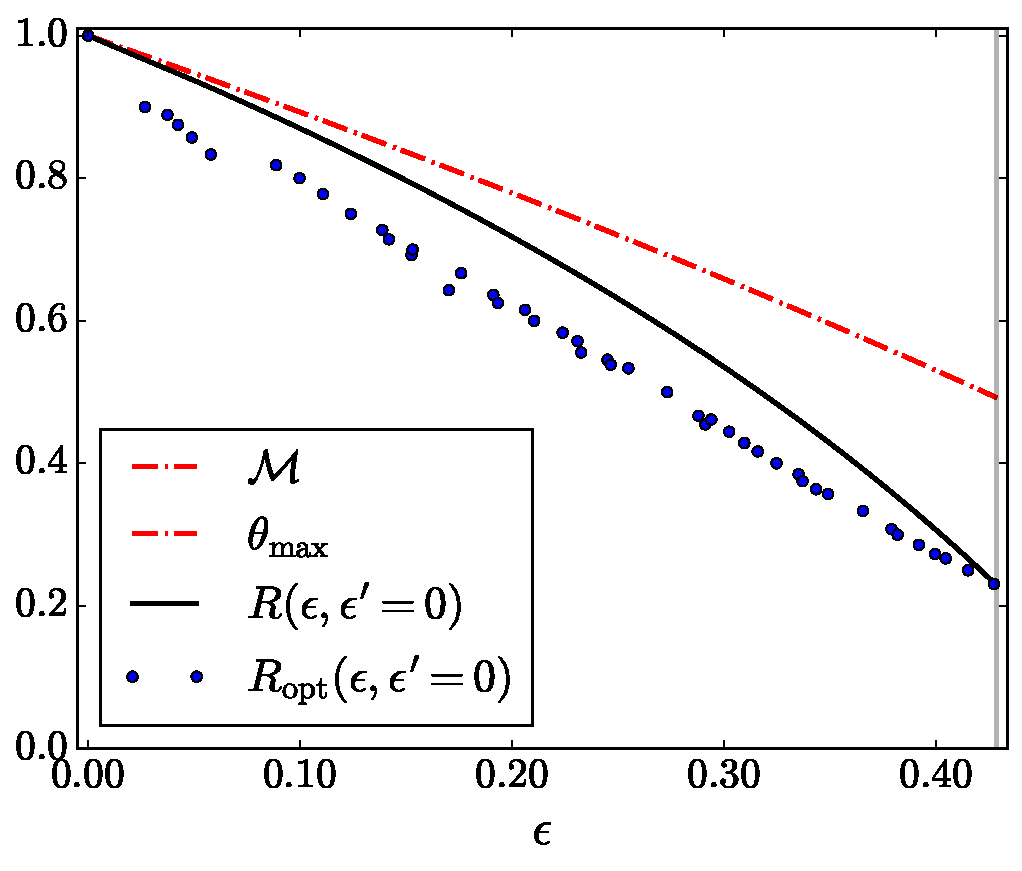
\includegraphics[scale=0.5]{figs/distill_bounds.pdf}
    \caption{\textbf{Distillation rate in unital fragment.} Distillation rates obtained by mana and majorization are plotted for $\epsilon' = 0$, up to noise levels $\epsilon_{\rm{max}} = \frac{3}{7}$.
    Majorization consistently provides stricter rates as proven in~\cref{thm:bounds}.
    }
    \label{fig:distill_bounds}
\end{figure}

\ddd{[Going forward:
\begin{enumerate}
\item Does the ``last elbow'' give the same bound? Is it as simple?
\item Numerically is this about as good as it gets from majorization?
\item How does this rate compare with existing literature?
\end{enumerate}
If this bound is better than existing literature then great. I suspect not though. However, remember the core message of our work is that we're ``incorporating physical restrictions'' into the magic analysis. Given this, one thing that would round the paper off could be if we re-played the ``first elbow'' bound for some non-trivial temperature. Meaning: choose a ``nice'' Hamiltonian and compute the first elbow constraint via the thermo-majorization distortion of the Wigner components. This would then give us something clearly new -- namely a bound with temperature dependence! People would find this interesting since nothing like it exists yet.}

\subsection{Magic in thermal fragments}\label{sec:thermal}

Consider a system driven by Hamiltonian $H$ and a circuit consisting of thermal operations.
The computational basis now coincides with the Hamiltonian eigenbasis.
We denote the thermal state at temperature $\beta^{-1}$ by $\gamma_\beta = \frac{e^{-\beta H}}{\Z_\beta}$, where $\Z_\beta = \tr[e^{-\beta H}]$.\nick{expand}

Thermal operations coincide with fragment $\O_{\gamma_\beta}$ \nick{expand}. \ddd{[Completely vital. What Hamiltonian are you choosing? Note you can choose it to make life easy for yourself. E.g. $H=Z$ for example.]}\nick{$X, Z$ are not Hermitian. Currently a general Hamiltonian with spectrum $(\epsilon_0,\epsilon_1,\epsilon_2)$.}
The Wigner distribution of any thermal state $\gamma_\beta$ is calculated directly by the definition in~\cref{eq:wstate},
\begin{equation}
	\W[\bmx]{\gamma_\beta} = \frac{e^{-\beta \epsilon_{x_0}}}{d\Z_\beta}\ \text{for all}\ \bmx \in \pd,
\end{equation}
and always consists of strictly positive components, so pre-order $\prec_{\gamma_\beta}$ is well defined.

Take the simplest scenario, where Hamiltonian $H$ has spectrum $(1,0,0)$.
Then, $\Z_\beta = 2 + e^{-\beta}$ and the 1-copy Wigner distributions are depicted in~\cref{tab:thermal_w}.
\begin{table}[h]
  \def\arraystretch{1.5}
  \centering
  \begin{tabular}{c|c|c|c}
    $\bmx = (x_0, x_1)$ & $W_{\noisys}(\bmx)$ & $W_{\gamma_\beta}(\bmx)$ & $W_{\noisys}(\bmx)/W_{\gamma_\beta}(\bmx)$ \\
    \hline
    $(0,0)$ & $-\frac{1}{3}$ & $\frac{1}{3(1+2e^\beta)}$ & $-\frac{1}{1+2e^\beta}$ \\
    \hline
    \makecell{$(0,1)$ \\ $(0,2)$} & $\frac{1}{6}$ & $\frac{1}{3(1+2e^\beta)}$ & $\frac{1}{2(1+2e^\beta)}$ \\
    \hline
    \makecell{$(1,0)$ \\ $\vdots$ \\ $(2,2)$} & $\frac{1}{6}$ & $\frac{1}{3(2+e^{-\beta})}$ & $\frac{1}{2(2+e^{-\beta})}$
  \end{tabular}
  \caption{Wigner components $W_{\gamma_\beta}(\bmx)$, $W_{\noisys}(\bmx)$ and their ratio $W_{\noisys}(\bmx)/W_{\gamma_\beta}(\bmx)$.
  The order of the ratio depends on temperature $\beta$ with a threshold value of $\beta_{\rm{thr}} \approx 0.48$.}
  \label{tab:thermal_w}
\end{table}
To construct the Lorenz curves, we need to sort the ratio $W_{\noisys}(\bmx)/W_{\gamma_\beta}(\bmx)$, but sorting depends on temperature $\beta$. 

\newpage

For a qutrit, let the energy spectrum be $E_0 \geq E_1 \geq E_2$. 
Then, we can explicitly write the thermal Wigner distribution as
\begin{equation}
	\W{\gamma_\beta} = \frac{1}{3\Z_\beta} \big( \overbrace{e^{-\beta E_0}}^3, \overbrace{e^{-\beta E_1}}^3, \overbrace{e^{-\beta E_2}}^3 \big),
\end{equation}
which is sorted in decreasing order.
We choose the Strange state where the negativity is in the first component of its Wigner distribution
\begin{equation}\label{eq:wsu}
	\W{\noisys(\epsilon)} = \Bigg( \overbrace{-\frac{1}{3} + \frac{4}{9}\epsilon}^1, \overbrace{\frac{1}{6} - \frac{1}{18}\epsilon}^8\Bigg),
\end{equation}

However, higher copies are not sorted, for example
\begin{equation}
	\begin{split}
	\W{\gamma_\beta\too{2}} = \frac{1}{9\Z_\beta^2} \Bigg( &\overbrace{\overbrace{e^{-\beta 2E_0}}^3, \overbrace{e^{-\beta (E_0 + E_1)}}^3, \overbrace{e^{-\beta (E_0 + E_2)}}^3}^3, \\
	 &\overbrace{\overbrace{e^{-\beta (E_1 + E_0)}}^3, \overbrace{e^{-\beta 2E_1}}^3, \overbrace{e^{-\beta (E_1 + E_2)}}^3}^3, \\
	 &\overbrace{\overbrace{e^{-\beta (E_2 + E_0)}}^3, \overbrace{e^{-\beta (E_2 + E_1)}}^3, \overbrace{e^{-\beta 2E_2}}^3}^3 \Bigg).
	\end{split}
\end{equation}
\ddd{[Definitely impressed by this Latexing...but perhaps just give the multiplicities and spectrum values. I.e. ``(blah) with multiplicity (blah) and ...'']} \nick{So the problem is that the exact position of each component matters, e.g. thermal state component $e^{-\beta 2E_0}$ corresponds to a positive Strange state component in one position and a negative Strange state component in another.} 
For the Strange state we have
\begin{equation}
	\begin{split}
	\W{\noisys(\epsilon)\too{2}} = \Bigg( &\overbrace{\left( -\frac{1}{3} + \frac{4}{9}\epsilon \right)^2}^1, \overbrace{ \left( -\frac{1}{3} + \frac{4}{9}\epsilon \right) \left( \frac{1}{6} - \frac{1}{18}\epsilon \right)}^{8}, \\
	&\overbrace{\overbrace{ \left( -\frac{1}{3} + \frac{4}{9}\epsilon \right) \left( \frac{1}{6} - \frac{1}{18}\epsilon \right)}^1, \overbrace{\left( \frac{1}{6} - \frac{1}{18}\epsilon \right)^2}^8}^8,  \Bigg).
	\end{split}
\end{equation}
\nick{We need to sort the distributions $\W{\gamma_\beta\too{2}}, \W{\noisys(\epsilon)\too{2}}$, so that the vector
\begin{equation}
	\tilde{\bm{w}} \coloneqq \left(\frac{(\W{\noisys(\epsilon)\too{2}})_1}{(\W{\sigma})_1}, \dots, \frac{(\W{\rho})_{81}}{(\W{\sigma})_{81}} \right)^T,
\end{equation}
is in decreasing order, i.e. $\tilde{\bm{w}} = \tilde{\bm{w}}^\downarrow$.
Then, we need to generalise for any number of copies $n$}

\null\newpage
\null\newpage

We generalise the analysis of unital fragments into any circuit with thermalisation noise parametrised by the temperature $\beta^{-1}$.
In~\cref{fig:thermal_distill}, we examine the majorization bound for the same purification process of~\cref{eq:sdist} with $\epsilon' = 0.05$.
The curves plotted suggest that there exists a fragment $\O_{\gamma_{\beta_{\rm{max}}}}$ which allows for a highest noise threshold at any given number of copies of the initial state.
Adding more copies results in a lower optimal temperature $\beta^{-1}$.

\begin{figure}[h]
    \centering
    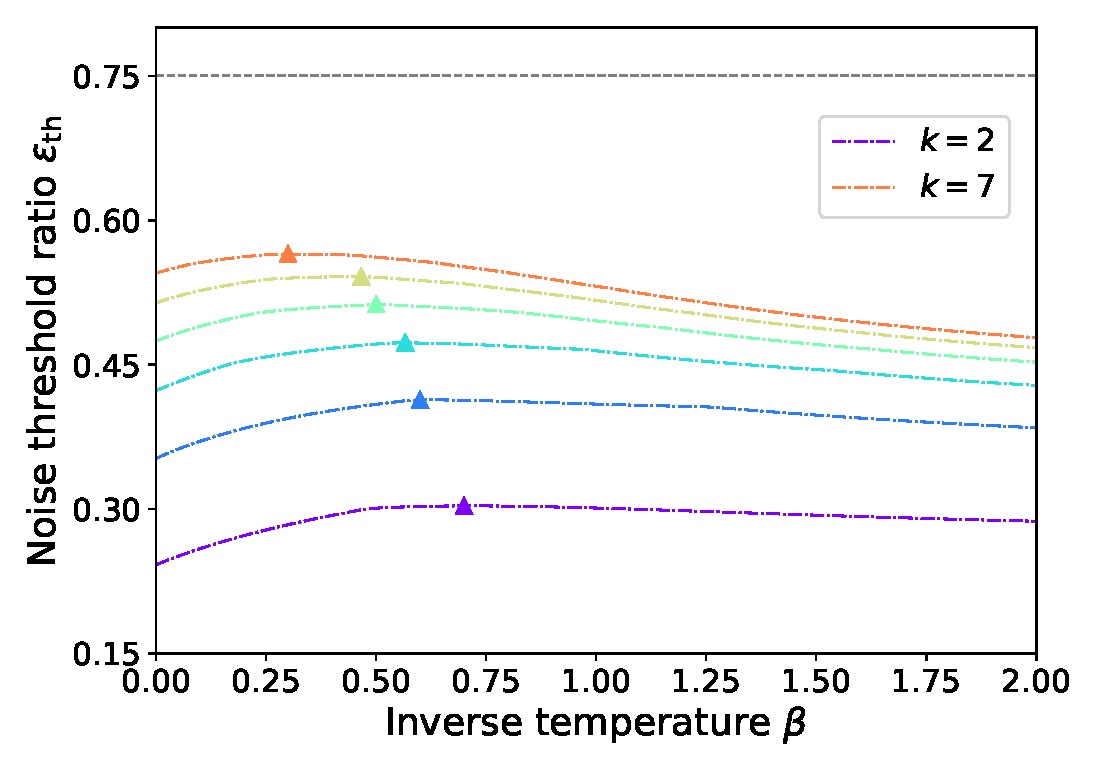
\includegraphics[scale=0.5]{figs/thermal_distill.pdf}
    \caption{\textbf{Threshold dependence on temperature in thermal fragments.} Lorenz curve ratios for the Strange state purifying process in~\cref{eq:sdist} with $\epsilon' = 0.05$.
    The peaks of each curve indicate the optimal temperature $\beta_{\rm{max}}$ that allows for the highest noise threshold at every given number of initial state copies $k$.
    The line $\epsilon = \frac{3}{4}$ indicates the threshold noise beyond which the Strange state no longer contains negativities.
    }
    \label{fig:thermal_distill}
\end{figure}

\subsection{Magic in pure stabilizer fragments}\label{sec:magstab}

There exist $d(d+1)$ pure stabilizer states for a $d$-dimensional system, all of which correspond to a uniform distribion over an affine line in the phase space \nick{CITE}.
As an example, the distribution of the qutrit zero state $\ketbra{0}$ is illustrated in~\cref{fig:zero}.
Any pure stabilizer state $\sigma$ is a rank--$1$ state and contains $d^2 - d$ zeros in its Wigner distribution, so we approximate it by the full--rank state $\sigma' = (1-\epsilon)\sigma + \epsilon \frac{1}{d}\id$ for some infinitesimal $\epsilon > 0$.

We explore the distillation process of~\cref{eq:sdist} in these modified fragments $\O_\sigma'$ in~\cref{fig:stab_distill}.
We repeat the plot for distillation of Norrell states in~\cref{fig:stab_distill_norrell}.


\begin{figure}[h]
    \centering
    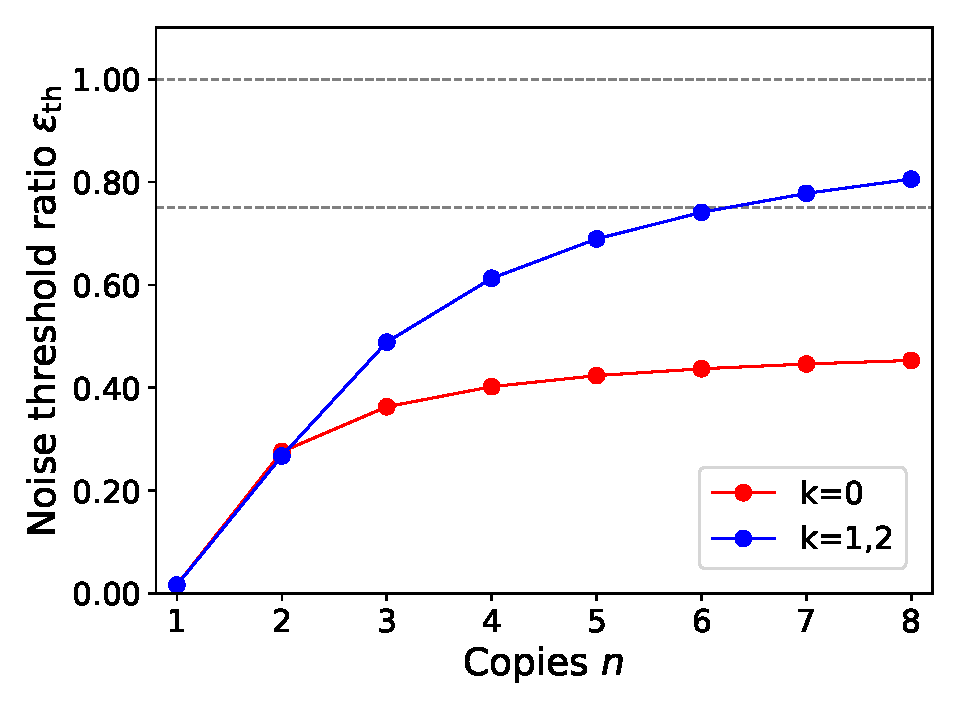
\includegraphics[scale=0.5]{figs/stab_distill.pdf}
    \caption{\textbf{Strange state distillation thresholds in stabilizer fragments.} Lorenz curve thresholds for the Strange state purifying process in~\cref{eq:sdist} with $\epsilon' = 0.05$.
    All $12$ stabilizer fragments produce two distinct trends: ($k=0$ - red curve) the stabilizer states that have non-zero value at the origin of the phase space lie low and ($k=1,2$ - blue curve) the stabilizer states that have a zero value at the origin of the phase space lie high.
    This is specific to the Strange state.
    For high enough copies, these Lorenz curves surpass the unital noise threshold $\epsilon_{\rm{th}} = \frac{3}{4}$.
    }
    \label{fig:stab_distill}
\end{figure}

\begin{figure}[h]
    \centering
    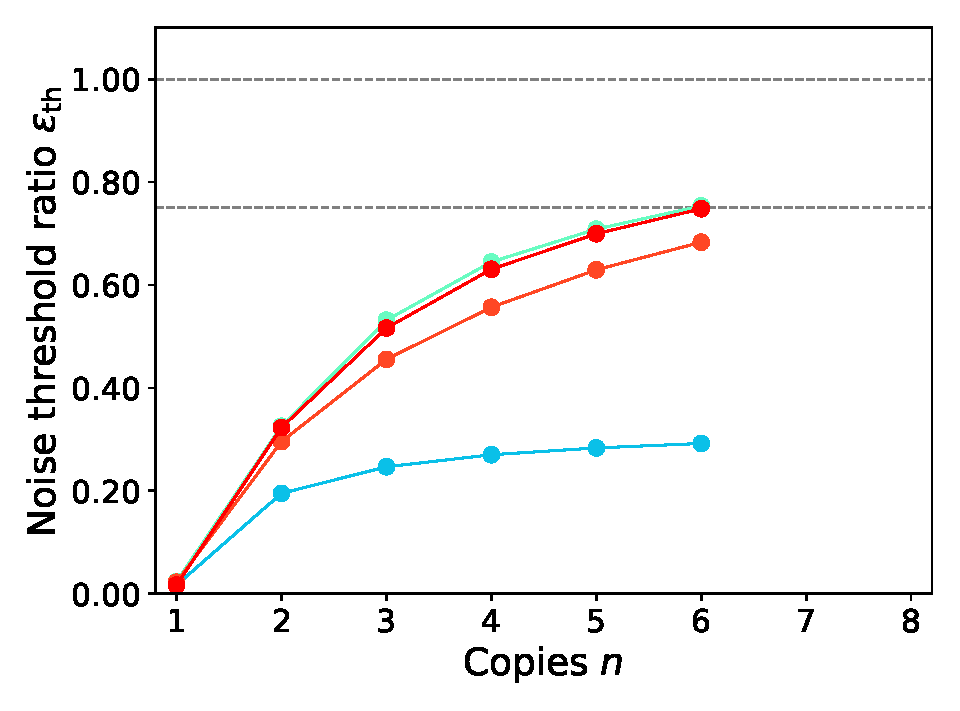
\includegraphics[scale=0.5]{figs/stab_distill_norrell.pdf}
    \caption{\textbf{Norrell state distillation thresholds in stabilizer fragments.} Lorenz curve thresholds for the Strange state purifying process in~\cref{eq:sdist} with $\epsilon' = 0.05$.
    For high enough copies, certain Lorenz curves surpass the unital noise threshold $\epsilon_{\rm{th}} = \frac{3}{4}$.
    }
    \label{fig:stab_distill_norrell}
\end{figure}

%%%%%%%%%%%%%%%%%%%%%%%%%%%%%%%%%%%%%%%%
\null\newpage
\section{Lower bounds in $\sigma$-fragments}
\ddd{[Am throwing down some rough material, to be polished later.]}

In order to obtain lower bounds one must now make precise what the free operations actually are in the  theory, beyond the condition of preserving Wigner-positivity.

We first consider the unital fragment, and consider the transformations possible using Clifford unitaries, and convex mixtures of Clifford unitaries. We denote the Clifford group as $\C$, and given some quantum state $\rho$ the accessible states in the unital fragment are given by $\E(\rho) = \sum_{g \in \C} p(g) U(g) \rho U(g)^\dagger$.

\subsection{Symplectic majorization of magic state Wigner distributions.}
We now exploit the the group structure, which leads to a more general notation majorization that has been extensively studied in the classical context, but to our knowledge has not yet been used in quantum information theory.

\begin{definition} Given a group $G$ that acts on a vector space $V$, we say that $\bmx$ \emph{$G$-majorises} $\bmy$ precisely when $\y \in H(\x)$, where $H(\x)$ is the convex hull of $\{g \x : g \in G\}$. We denote this as $\y \prec_G \x$.
\end{definition}

Now any quantum state $\rho$ has a Wigner distribution $W_\rho(\x)$. Given a Clifford unitary $\U \in \C$ we have that its representation in the Heisenberg-Weyl frame is given by
\begin{equation}
W_{\U(\rho)} (\x) = [\mbox{\ddd{fill in}}].
\end{equation}

This group action corresponds to the action of the affine symplectic group on the discrete phase space $\P_d$. To proceed we can study the discrete translational action, and the symplectic action separately.

\subsection{Cyclic majorization conditions.}
We can consider for $G$, the cyclic group of order $N$, which is described by $G= \< g | g^N = e\>$. in Terms of the Wigner distributions, this arises for the discrete lattice translations arising from displacement operators.

A set of necessary and sufficient conditions for cyclic majorization has been obtained and is given as follows. Suppose $\x, \y$ are two real vectors in $\mathbb{R}^n$. Let $\Delta$ be the elementary shift operator, defined by
\begin{equation}
\Delta \x = \Delta (x_1, x_2, \dots, x_n) := (x_n, x_1, x_2, \dots, x_{n-1}),
\end{equation}
and from this it is clear that $\Delta$ generates a representation of the abelian group $(\mathbb{Z}_n,+)$.
We now say that $\x$ \emph{cyclically majorizes} $\y$, written $\x \succ_C \y$, if and only if 
\begin{equation}
\y = \sum_{k=0}^{n-1} p_k \Delta^k \x,
\end{equation}
for some probability distribution $p=(p_k)$. This means that $\y$ lies in the convex hull of the orbit of $\x$ under cyclic shifts. Thus, we may write this condition as $\y = L(\p) \x$, where
\begin{equation}
L(\p) :=  \sum_{k=0}^{n-1} p_k \Delta^k,
\end{equation}
is a linear operator, as a function of an unknown distribution $\p$. We now have the following key identity for linear operators of this form:
\begin{equation}
L(\p)\x = QL(\x) \p,
\end{equation}
where $Q$ is a permutation matrix sending $e_0:=(1,0,0,\dots ,0)$ to itself, and otherwise sending $e_k$ to $e_{n-1-k}$, where $e_k=  (0,0,\dots, 0,1,0,\dots, 0)$ is the $k$'th basis vector. We thus have
\begin{align}
\x \succ_C \y &\Leftrightarrow \y = L(\p) \x \mbox{ for some dist. } \p. \nonumber \\
&\Leftrightarrow \y = QL(\x) \p \mbox{ for some dist. } \p. \nonumber \\
&\Leftrightarrow [QL(\x)]^{-1}\y = \p \mbox{ for some dist. } \p. \nonumber \\
&\Leftrightarrow [QL(\x)]^{-1}\y = \p  \ge \mathbf{0} \mbox{ and normalized}.
\end{align}
This implies that to check whether $\x \succ_C \y$ it suffices to compute the components of the left-hand side and ensure non-negativity (I suspect it is normalised if $\x$ and $\y$ are normalised).

Note though that by using Fourier analysis we can simplify this in terms of computational demands to checking if the vector
\begin{equation}
\p = C(\x') Q\y,
\end{equation}
has non-negative components, where
\begin{equation}
\x' := n\F_n [\F_n\x]^{-1},
\end{equation}
with $\F_n$ being the discrete Fourier transform, and the bracket term $[\F_n \x]^{-1}$ denotes the vector obtained by inverting the components of $\F \x$ individually. So the recipe for cyclic majorization is:
\begin{enumerate}
\item Given inputs $\x$ and $\y$.
\item Compute the vector $\x'$ via two Fourier transforms and $n$ inversions.
\item Compute the circulant matrix $C(\x')$.
\item Compute $\C(\x')Q \y$ and check if all components are non-negative.
\end{enumerate}•


\subsection{Symplectic majorization for qutrit magic}
The qutrit system provides a good illustration of the techniques. In this case the symplectic group $SL(2,\mathbb{Z}_3)$ is isomorphic (up to $\pm \I$) the symmetry group of the tetrahedron, which in turn is isomorphic to $S_4$, the permutation group on 4 symbols. Therefore we expect in this case that symplectic majorization on $\P_3$ corresponds to a restricted form of majorization.


\subsection{Fundamental Regions of a group $G$}
\ddd{[This is theory for the appendices, and also to help flesh out the theory of $G$ majorization. It looks a bit technical, but the core idea is simple enough once you get it.]}
Given a group $G$ that acts on a vector space $V$, we now have the following concept.
\begin{definition} A \emph{fundamental region} $F$ of $G$ in $V$ is any open set $F$ such that $F \cap gF = \varnothing$ for $g \ne e$ and moreover 
\begin{equation}
V = \bigcup_{g} \overline{g F}.
\end{equation}
\end{definition}
Here, the overline denotes the closure of a set. Loosely speaking, we can view $F$ as obtained by quotienting the vector space $V$ via the group action. We then have the following key theorem, which is proved in [CITE].
\begin{theorem} If $G$ has a fundamental region $F$ that is unique, modulo actions of the group $F\rightarrow gF$, then $\bar{F}$ is a closed, convex cone and for any $\x, \y \in \bar{F}$ we have
\begin{equation}
\y \prec_G \x \Leftrightarrow \mathbf{a}\cdot \y \le \mathbf{a} \cdot \x, \mbox{ for all } \mathbf{a} \in \bar{F}.
\end{equation}
\end{theorem}
If the cone $\bar{F}$ is finitely generated, namely 
\begin{equation}
\bar{F} = \mbox{cone}( \mathbf{c}_1, \dots, \mathbf{c}_N),
\end{equation}
for some finite set of vectors, then the majorization condition reduces to checking a \emph{finite} set of inequalities, namely checking $\mathbf{c}_k \cdot \y \le \mathbf{c}_k \cdot \x$ for $k=1, \dots , N$.

Note now that any group action $G$ on a vector space $V$ always has a fundamental region. Consider any $\x \in V$ such that $g \x \ne \x$ unless $g =e$. For this we define
\begin{equation}
K = \{ \mathbf{a} \in V : \sup_g \left [ (g\mathbf{a})\cdot \x \right ] = \mathbf{a} \cdot \x \},
\end{equation}
then $F = K_{\mbox{\tiny int}}$ is a fundamental region of $G$ in $V$, where $ K_{\mbox{\tiny int}}$ is the interior of the set $K$. In simple terms, this fundamental region corresponds to the set of vectors that are `close' to $\x$, in the sense that any non-trivial group action $\mathbf{a} \rightarrow g \mathbf{a}$ on them moves them away from $\x$ with respect the inner product. See [CITE] for a proof of this statement.

\subsection{Computing the fundamental region $F$ for the qutrit}
Firstly, note that we actually have that $SL(2, \mathbb{Z}_3)$ is represented by $U(g)$ on $\P_3$, and so we should use that notation for precision.

Since the symplectic group for $d=3$ is a reflection group, it turns out that this guarantees that an essentially unique fundamental region exists, and so we can reduce to a \emph{finite} set of majorization conditions (I think 5 in this case). Note that the $K$ defined above is always a closed, convex cone. This means it should be `easy' to determine the fundamental region. Reflection groups are Coexter groups, and I believe this set $K$ is essentially a Weyl chamber in that language. Anyhow, let's not get distracted by abstraction.


The concrete recipe going forward:
\begin{enumerate}
\item Pick your favorite $\x \in P_3$ that is \emph{not} stabilized by $g\ne e$. I.e. a vector that moves under all non-trivial group actions.
\item For each $g_k$ look for the extremal cases of $\y$ such that have constant inner product with $\x$. This corresponds to 
\begin{equation}
\left [ (U(g_k) -\I) \y \right ] \cdot \x = 0 \mbox{ for }k=1, \dots ,24.
\end{equation}
Or equivalently,
\begin{equation}
\y \cdot A^T\x = 0,
\end{equation}
where $A := U(g_k) -\I$.
\item Write down the matrix equation for each $g_k$.
\item Each of these conditions defines a hyperplane $H_k$ in $\P_3$ corresponding to the boundary of $K$.
\item We possibly don't need to range over all 24 group elements....but am not sure on this.
\item From this, we should be able to extract a generating set of vectors.
\end{enumerate}

\subsection{Toy example to see how the algorithm works}
Okay, let's see how it works in a simple case. Let's consider the case of $V= \mathbb{R}^2$ and $G=S_2=\<g|g^2=e\>$ with the group action $g.(x,y) = (y,x)$ that swaps the components of the vector. We should get standard majorization out of this $G$--majorization.

First we find an $\x$ that transforms non-trivially under non-trivial group actions. The vector $\x=(1,0)$ does this. To construct a fundamental region we now look at the equation 
\begin{equation}
[g.(x,y) - (x,y)] \cdot (1,0) = 0
\end{equation}
and solve for $x,y$. This becomes,
\begin{equation}
(y-x, x-y)\cdot(1,0)=0,
\end{equation}
which implies the hyperplane (line!) $y=x$ is the \emph{boundary} of the fundamental region. Since we decided to start with $(1,0)$ we can take the region to the right of this line, and so:
\begin{equation}
F = \{(x,y) : x>y \}
\end{equation}
where we note that we use the strict inequality to get the interior. The region $\bar{F}$ is a half-space, but this is actually a cone, and can be written as
\begin{equation}
F= \mbox{cone}( (1,1),(-1,-1), (5,0)).
\end{equation}
The first two vectors give the boundary, and we just need one other vector inside $F$ to generate it fully, chosen arbitrarily to be $(5,0)$. This last one is needed since $(1,1)$ and $(-1,-1)$ are linearly dependent! Therefore
\begin{align}
\mathbf{c}_1 &= (1,1) \nonumber \\
\mathbf{c}_2 &= (-1,-1) \nonumber \\
\mathbf{c}_3 &= (5,0).
\end{align}
The $S_2$--majorization ordering is then given by
\begin{equation}
\y \prec \x \Leftrightarrow \mathbf{c}_k \cdot \y \le  \mathbf{c}_k \cdot \x,
\end{equation}
for $k=1,2,3$ whenever $\x,\y \in F$. Note that is gives the ordering for all vectors in the space, since any general vector can be transformed into $F$ via a group action, since $F$ is a fundamental region. Indeed mapping an $\x$ into $F$ is simply $\x \rightarrow \x^\downarrow$, the sorting maneuver!
The generating vectors $(1,1)$ and $(-1,-1)$ imply that both 
\begin{equation}
y_1 + y_2 \le x_1 +x_2,
\end{equation}
and
\begin{equation}
y_1 + y_2 \ge x_1 +x_2,
\end{equation}
which becomes the majorization condition
\begin{equation}
y_1+y_2 = x_1 + x_2.
\end{equation}
Easy! The final condition from $\mathbf{c}_3=(1,0)$ is then the condition that
\begin{equation}
5y_1 \le 5x_1 \Rightarrow y_1 \le x_1,
\end{equation}
which is the final majorization condition. Thus we have shown how the familiar majorization structure corresponds to the theory of $G$--majorization, and the cone ordering structure that comes from fundamental regions.

\subsection{Another toy example -- non-standard majorization this time}
Okay, let's look at another option for $V=\mathbb{R}^2$. Now consider the group $G=\mathbb{Z}_2 \times \mathbb{Z}_2$ that can be represented as $G=\<g_1,g_2 | g^1=e, g_2 = e, g_1g_2 = g_2g_1\>$, and acts on vectors as $g_1.(x,y) = (-x,y), g_2.(x,y)=(x,-y)$. In other words the group just flips vectors about X/Y axes.

A vector that moves under the non-trivial group actions is $(1,1)$, so we use this one and solve for $[g.(x,y) - (x,y)] \cdot (1,1) = 0$. We have for $g = g_1$ the equation
\begin{equation}
[(-x,y) - (x,y)]\cdot (1,1) = 0,
\end{equation}
which implies the line $x=0$.

For $g=g_2$ we have
\begin{equation}
[(x,-y) - (x,y)]\cdot (1,1) = 0,
\end{equation}
which implies the line $y=0$.

For $g=g_1g_2$ we have
\begin{equation}
[(-x,-y) - (x,y)]\cdot (1,1) = 0,
\end{equation}
which implies the line $x+y=0$. The open region bounded by these three conditions is the set
\begin{equation}
F := \{ (x,y) : x>0, y>0\}.
\end{equation}
So the positive quadrant of $\mathbb{R}^2$ is a fundamental region for $G$, which makes sense since via sign flips we can map this onto the whole plane, once we close the set. This is again a convex cone and $\bar{F} = \mbox{cone}((1,0), (0,1))$. Thus given any two vectors $\x,\y$ we first act with $G$ to flip their signs so that their components are all positive, $\x \rightarrow \x^\star\ge \mathbf{0}$, then $\y \prec_G \x$ if and only if $y_1 \le x_1$ and $y_2 \le x_2$. This implies that 
\begin{equation}
\y \prec_G \x \Leftrightarrow \y^\star \le \x^\star. 
\end{equation}
So the $G=\mathbb{Z}_2 \times \mathbb{Z}_2$ majorization gives the component-wise ordering on vectors once you sort them. It is clear that this extends to any $G=\mathbb{Z}_2^{\times n}$.
\subsection{A more complex example $S_3$ on $\mathbb{R}^3$.}
So the symmetric group $S_n$ always gives majorization. But the symmetric group has $|S_n| = n!$ elements to it, which is super-exponentially big in $n$. We clearly don't have to check $n!$ equations, since the majorization conditions involve just $n+1$ inequalities, and so it must be that the basic generating conditions of the group suffice to determine the fundamental region of $G$.

Let's look at $V = \mathbb{R}^3$ and $G=S_3$ acting on $\x = (x_i)$ as $g.\x = (x_{g^{-1}}(i))$. A vector that transforms non-trivially under all non-trivial actions is $(2,1,0)$. Let's look at the transpositions, and the boundary planes they give first.

For $g= (1\,\,2)$ we have the equation
\begin{equation}
[(y,x,z) - (x,y,z)] \cdot (2,1,0) = 0,
\end{equation}
which implies the plane $2(y-x)+ x-y = 0$, namely,
\begin{equation}
H_1 = \{(x,y,z) : y=x\}.
\end{equation}
The other choices of transpositions work the same and give the planes
\begin{align}
H_2 &= \{(x,y,z) : y=z\} \\
H_3 &= \{(x,y,z) : x=z\}.
\end{align}
Note that their intersection gives the line $\{(x,y,z) : x=y=z\}$, which is the line of uniform vectors at the bottom of the majorization pre-order.

What information do the $3$-cycles give? Okay, let's now look at $g=( 1 \,\, 2 \,\, 3)$. The core equation for this becomes
\begin{equation}
[(z,x,y) - (x,y,z)] \cdot (2,1,0) = 0,
\end{equation}
and so gives
\begin{align}
2(z-x) + (x-y) &= 0 \nonumber \\
\Rightarrow x+y &=2z. 
\end{align}
Namely the plane
\begin{equation}
H_4 = \{(x,y,z) :  x+y =2z\}.
\end{equation}The remaining $3$--cycle $(3\,\,2\,\,1)$ gives
\begin{align}
H_5 &= \{(x,y,z) : y+z = 2x\}.
\end{align}
Note that $|S_3| = 6$, but the identity element $g=e$ gives no constraint, and so there are exactly $5$ bounding planes. Note also that the line $\{ (t,t,t)\} $ is again the intersection of all the planes.

These 5 planes bound a cone containing $(2,1,0)$, namely the fundamental region $F$. What's a good algorithm to obtain a generating set of vectors for this cone?

Firstly, since the line $\{(t,t,t)\}$ being the intersection of all the planes, is definitely on the boundary of $F$, this means we must have $\mathbf{c}_1 = (1,1,1)$ and $\mathbf{c}_2 = (-1,-1,-1)$ in our generating set. Perhaps a good algorithm is to compute intersections, obtain generating vectors for these intersections of the hyperplanes, $H_{ij}$ and then let $K_i$ and $K_j$ be the half-spaces in which $(2,1,0)$ resides. Now the intersection of two cones, is itself a cone so we can just keep intersecting the half-space/cones. Thus, we compute
\begin{align}
H_{12} &:= H_1 \cap H_2 \\
&=\{ (t,t,t) : t\in \mathbb{R}\}=:L.
\end{align}
Similarly, $H_{13} = H_{23}= L$. What about the other intersections? Well $H_{14} = H_{15}=L$. In fact all intersections are the same! 
\begin{equation}
H_{ij} = H_i \cap H_j = L \mbox{ for all } i,j.
\end{equation}
The fundamental region is given by the intersection of $K_1$ and $K_2$, or any other two half-spaces. This is generated by $\mathbf{c}_1$ and $\mathbf{c}_2$ above, and any two independent vectors in the intersection of these half-spaces. We can choose 
\begin{align}
\mathbf{c}_3 &= (1,1,0) \\
\mathbf{c}_4 &= (1,0,0),
\end{align}
note that $\mathbf{c}_3 \in H_1$ and $\mathbf{c}_4 \in H_2$, while $\mathbf{c}_3 \in K_2$ and $\mathbf{c}_4 \in K_1$ and so this works correctly. We thus have
\begin{equation}
\bar{F} = \mbox{cone}(\mathbf{c}_1 ,\mathbf{c}_2 ,\mathbf{c}_3 ,\mathbf{c}_4 ).
\end{equation}
The first two inequalities give the condition that
\begin{equation}
x_1+x_2+x_3 = y_1+y_2+y_3,
\end{equation}
while the remaining two conditions give the inequalities
\begin{align}
y_1 &\le x_1 \\
y_1+y_2 &\le x_1 +x_2.
\end{align}
This is the standard majorization relation. Geometrically, the cone $\bar{F}$ is actually a funny one to visualise: it consists of a half-line radiating out from $(0,0,0)$ to $(-1, -1, -1)$, together with the triangular ``infinite pyramid'' generated by positive combinations of $(1,1,1), (1,1,0), (1,0,0)$. But we can also take positive linear combinations of $(-1,-1,-1)$ and e.g. $(1,1,0)$ and so it is still a bit tricky to visualise.
\subsection{Symplectic majorization for $d =5$ and beyond.}
For the case $d=5$ we also have a particularly simple group structure, where now the symplectic group $SL(2, \mathbb{Z}_5)$ is isomorphic to the symmetry group of the icosahedron. This is another reflection group and therefore we can again obtain the finite set of majorization conditions to describe it. Here the order of the group is $60$ and so we probably shouldn't make Nick compute this by hand.
\newpage
\section{Extension to general quantum resource theories}
\label{sec:frag}

In the previous section we introduced the notion of $\sigma$--fragments for any resource theory of magic. In this section we pause to generalise this concept to an arbitrary resource theory and explain precisely how it connects with resource monotones. The busy reader more focussed on magic may skip this section. \nick{restate}

State convertibility within a given resource theory is often a hard question to address due to the intricate structure of the theory.
In general, the structure of a theory $\R$ is described by a pre-order $\prec_\R$ and usually resource monotones are employed to reduce this structure into a simple real number ordering\nick{CITE}.
The subdivisions of magic theories into $\sigma$--fragments suggests a new approach towards investigating state convertibility which retains more structure of the origin theory than a measure can.

Monotones reduce the structure of the resource theory $\R$ to a \emph{total} order on the real numbers.
Therefore, two states, even if incomparable in $\R$, are always mapped onto ordered real numbers.
We now generalise this idea of a theory projection that preserves comparability between states. 
\begin{definition}[\textbf{Covariant projection}]\label{def:covproj}
Let $\R = (\F, \O)$ be a resource theory with pre-order $\prec_\R$. 
Then a \emph{covariant resource projection} of $\R$ to a resource theory $\R'$ with pre-order $\prec_{\R'}$, is a pair of mappings $(\Pi_s, \Pi_o)$, where $\Pi_s$ maps quantum states in $\R$ to quantum states in $\R'$, and $\Pi_o$ maps free operations in $\R$ to free operations in $\R'$. 
Moreover, these obey
	\begin{enumerate}
        \item $\Pis(\rho_1) \prec_{\R'} \Pis(\rho_2)$ whenever $\rho_1 \prec_\R \rho_2$;
        \item $\Pio(\E) = \Pio(\E_1) \circ \Pio(\E_2)$ whenever $\E = \E_1 \circ \E_2$.
    \end{enumerate}
We call $\R'$ a \emph{covariant fragment} of $\R$.
\end{definition}

Resource monotones can now be clearly seen as a special case of covariant resource projections.
\begin{proposition}[\textbf{Totally ordered covariant theories}]\label{thm:monoproj}
	Any resource monotone $\M$ of a resource theory $\R$ is a covariant projection for which $\prec_{\R'}$ is a total order. 
	Conversely, any such covariant projection corresponds to a resource monotone $\M$. 
\end{proposition}
\begin{proof}
	Consider a monotone $\M$ in the context of a general resource theory $\R = (\F, \O)$.
	State order is covariantly preserved due to the defining property of a monotone, stated in~\cref{def:mono}, where the pre-order $\prec_{\R'}$ is simply the total order $\leq$ on $\mathbb{R}$. 
	
	Operational composition is covariantly preserved when we simply choose $\Pio(\E) = 1_\times$, namely the `multiplication by 1' operation on real numbers. 
	The definition of a resource monotone then automatically implies covariance.
	
	Conversely, given any covariant projection of $\R$ for which $\prec_{\R'}$ is a total order, we may map the totally ordered set of elements $\Pis(\rho)$ via an injective, non-decreasing function $f$ into $\mathbb{R}$. 
	Then, $\M(\rho):=f(\Pi_s(\rho))$ provides a numerical value for each $\rho$ that obeys the definition of a monotone.
	
\end{proof}

We can also view $\sigma$--fragments as an example of reducing the structure of a magic theory $\R$ to a subtheory with a tractable pre-order.
However, states which are incomparable in $\R$ remain incomparable and conversions between states which are comparable in $\R$ may no longer be possible.
\begin{definition}[\textbf{Contravariant projection}]\label{def:contraproj}
	Let $\R = (\F, \O)$ be a resource theory with pre-order $\prec_\R$. 
Then a \emph{contravariant resource projection} of $\R$ onto a resource theory $\R'$ with pre-order $\prec_{\R'}$, is a pair of mappings $(\Pi_s, \Pi_o)$, where $\Pi_s$ maps quantum states in $\R$ onto quantum states in $\R'$, and $\Pi_o$ maps free operations in $\R$ onto free operations in $\R'$. 
Moreover, these obey
	\begin{enumerate}
        \item $\rho_1 \prec_\R \rho_2$ whenever $\Pis(\rho_1) \prec_{\R'} \Pis(\rho_2)$;
        \item $\E = \E_1 \circ \E_2$ whenever $\Pio(\E) = \Pio(\E_1) \circ \Pio(\E_2)$.
    \end{enumerate}
We call $\R'$ a \emph{contravariant fragment} of $\R$.
\end{definition}
The use of covariant and contravariant in~\cref{def:covproj,def:contraproj} refers to the direction of implication between the two pre-orders and operation compositions\footnote{Note that strictly these are not projections in the sense of $\Pi^2 = \Pi$, but are instead morphisms. 
Here our use of the term projection is motivated by the idea that one one generally loses information about $\R$ under the mapping.}.

\nick{Perhaps scrap definition of contravariant projection and define contravariant fragment as a subtheory $\R'$ where there exists a (injective) covariant projection from $\R'$ to parent theory $\R$. That would make every subtheory $\R' = (\F', \O')$ a contravariant fragment if $\O'$ is closed under composition, this includes $\sigma$--fragments.}

\begin{proposition}\label{thm:subproj}
    Let $\R = (\F, \O)$ be a resource theory, and let $\O' \subseteq \O$ be a non-empty subset of the free operations that is closed under composition, and moreover $\O'$ is the largest such subset, in the sense that for any $\E_1 \not \in \O'$ and any $\E_2 \in \O'$ we have that both $\E_1 \circ \E_2$ and $\E_2 \circ \E_1$ are not in $\O'$. Then $\R' = (\F, \O')$ of $\R$ defines a contravariant fragment of $\R$.    
\end{proposition}
\begin{proof}
    We first define $\Pis (\rho) = \rho$ for all $\rho$. It is clear that since $\O'$ is a subset of $\O$ any operation in $\O'$ will map the set of free states into itself. Moreover the identity channel $id$ is necessarily in $\O'$, due to the maximality assumption. For $\Pio$ we let $\Pis(\E) = \E$ if $\E \in \O'$ and otherwise $\Pis(\E) =id$. Now consider $\Pio (\E_1 \circ \E_2)$. Either the triple $\{\E_1, \E_2, \E_1\circ \E_2\}$ are all in $\O'$ or they are all outside of $\O'$. For the former case $\Pio(\E_1 \circ \E_2) = \E_1 \circ \E_2 = \Pio(\E_1) \circ \Pio(\E_2)$, while for the latter $\Pio(\E_1 \circ \E_2) = id = \Pio(\E_1) \circ \Pio(\E_2)$, which proves that compositions are respected under the map. Finally, $\rho \prec_{R'} \sigma$ implies there exists $\E \in \O' \subseteq \O$ such that $ \E(\rho) = \sigma$, and since $\E \in \O$ this implies $\rho \prec _{\R} \sigma$, as required, which completes the proof.
    
\end{proof}
\nick{Suppose $\E_2$ is the replacement channel $\E_2(\rho) = \sigma$. This is a stabilizer operation. Then $\E_2 \circ \E_1 \in \O_\sigma$ even if $\E_1 \notin \O_\sigma$. Now suppose $\E$ is a Hadamard unitary, then $id = \E \circ \E_{reverse}$ but $id \in \O_{\ketbra{0}}$ while $\E, \E_{reverse} \notin \O_{\ketbra{0}}$.} \ddd{[Ah ok, agreed. This is fine for now. Let's not spend ages trying to generalise this so as to include the majorization fragments. It's just good to explore the possibilities a bit, to illustrate the non-trivial aspects.]}
As an immediate corollary of~\cref{thm:subproj}, a $\sigma$--fragment of any magic theory $\R$ is a contravariant fragment of $\R$.


\begin{proposition}
	Let $\R = (\F,\O)$ be a resource theory, and let $\D \in \O$ be a free operation, which is reversible by $\D_{\rm{rev}} \in \O$, so that $\D_{\rm{rev}} \circ \D = \idc$.
	
	Then, we can define a contravariant projection of $\R$, by acting on all quantum states with $\D$.
\end{proposition}
\begin{proof}
	We show that the theory $\R' = (\F', \O)$, with $\F' = \{\D(\rho):\rho \in \F \}$, is a contravariant fragment of $\R$.
	
	Let $\Pis$ map every state $\rho$ to $\D(\rho)$ and suppose $\D(\rho_1) \prec \D(\rho_2)$. 
	Then, there exists $\E \in \O$ such that $\rho_1 = (\D_{\rm{rev}} \circ \E \circ \D) (\rho_2)$, so $\rho_1 \prec \rho_2$.
	
	Finally, let $\Pio$ map every free operation to itself, so that composition of operations is trivially preserved.
	
\nick{If $\D$ is a recovery map, so that $\D \circ \D_{\rm{rev}} = \idc$, then this is a covariant projection instead.

If $\D$ is not reversible, this mapping is in general NOT contravariant (consider the replacement map $\D(\rho) = \frac{1}{d}\id$ for a strange state and stabilizer state - surely there is such a counterexample in thermodynamics theory if we consider a highly coherent state and one with the same energy population but no coherences.} \ddd{[Ok. Again, let's not spend time worrying about this now. It's clear there is various fine-print to these cases...but they're not essential to our work so let's put this on hold.]}
\end{proof}

Important examples of resource fragments appear in several established resource theories. \nick{Need to check if the thermodynamics example works, include magic theories as fragments of $\Rmax$, include Nielsen's bipartite entanglement.} \ddd{[Don't worry about these things now -- let's get the computations section improved]}

\newpage

%%%%%%%%%%%%%%%%%%%%%%%%%%%%%%%%%%%%%%%%

\section{Conclusion}
\label{sec:conc}

\begin{enumerate}
    \item Introduced fragments
    \item Identify symmetries of the setup
    \item Combined single-shot thermodynamics with magic 
    \item Can we solve other cases exactly? (apart from single qutrit)
\end{enumerate}

%%%%%%%%%%%%%%%%%%%%%%%%%%%%%%%%%%%%%%%%

\bibliography{bib}
%\bibliographystyle{apsrev4-2}

%%%%%%%%%%%%%%%%%%%%%%%%%%%%%%%%%%%%%%%%

\appendix
\section{Properties of majorization}
\label{app:major}

\subsection{Equivalent conditions for majorization}

\begin{theorem}
Given $\bmx, \bmy, \bmd \in \mathbb{R}^n$, such that the components of $\bmd$ are positive, the following statements are equivalent:
 \begin{enumerate}
	\item[(TM1)] $\bmx \prec_{\bmd} \bmy$;
	\item[(TM2)] $\Gamma_{\bmd}({\bmx}) \prec \Gamma_{\bmd}({\bmy})$;
	\item[(TM3)]\label{en:tm3} $\sum\limits_{i=1}^n \abs{x_i - t d_i} \leq \sum\limits_{i=1}^n \abs{y_i - t d_i}$ for all $t \in \mathbb{R}$;
	\item[(TM4)] $\sum\limits_{i=1}^n (x_i - t d_i)^+ \leq \sum\limits_{i=1}^n (y_i - t d_i)^+$ for all $t \in \mathbb{R}$ and $\sum\limits_{i=1}^n x_i = \sum\limits_{i=1}^n y_i$;
	\item[(TM5)] $\forall k, L_{\bmx|\bmd}(k) \leq L_{\bmy|\bmd}(k)$ and $L_{\bmx|\bmd}(k=n) = L_{\bmy|\bmd}(k=n)$.
 \end{enumerate}
\end{theorem}
\begin{proof}
    \begin{enumerate}
        \item[1$\leftrightarrow2$]
        Suppose now there exists a stochastic $S$ such that $\bmx = S\bmy$ with $\bmd = S\bmd$ and let $B = \Gamma_{\bmd} \circ S \circ \Gamma_{\bmd}^{-1}$.
        $B$ is a $D$-dimensional bistochastic matrix, since composition of stochastic matrices is stochastic and $(\Gamma_{\bmd} \circ S \circ \Gamma_{\bmd}^{-1}) (\frac{1}{D}\bm{1}) = (\Gamma_{\bmd} \circ S) (\bm{d}) = \Gamma_{\bmd}(\bm{d}) = \frac{1}{D}\bm{1}$. Then, $B$ maps $\Gamma_{\bmd}({\bmy})$ to $\Gamma_{\bmd}({\bmx})$.
        Conversely, given $B$, let $S = \Gamma_{\bmd}^{-1} \circ B \circ \Gamma_{\bmd}$.
        Similarly, $S$ is the stochastic matrix that preserves $\bmd$ and maps $\bmy$ to $\bmx$.
        \item[$2\leftrightarrow3$]\hspace{-5pt}, $2\leftrightarrow4$, $2\leftrightarrow5$ These three statement are equivalent to \nick{blah} respectively for the embedded vectors $\Gamma_{\bmd}({\bmx}), \Gamma_{\bmd}({\bmy})$.
        This is clear by rewriting
        \begin{align}
            \sum\limits_{i=1}^n \abs{x_i - t d_i} &= \sum\limits_{i=1}^n d_i \abs{\frac{x_i}{d_i} - t} = \sum\limits_{i=1}^D \abs{\Gamma_{\bmd}(\bmx)_i - t}, \\
            \sum\limits_{i=1}^n (x_i - t d_i)^+ &= \sum\limits_{i=1}^D (\Gamma_{\bmd}(\bmx)_i - t)^+, \\
            L_{\bmx|\bmd}(k) &= L_{\Gamma_{\bmd}(\bmx)}(k'), \\
            \text{with}\ k&=1,\dots,n\ \text{and}\ k'=1,\dots,D \nonumber
        \end{align} 
        and similarly for the right hand side.
    \end{enumerate}
\end{proof}

\subsection{Mana properties}
Mana monotonicity can be directly seen due to statement~\ref{en:tm3} in~\cref{thm:dmajor} for $t=0$.
Furthermore, mana is additive due to the multiplicative property~\ref{en:w4} of~\cref{thm:wstate}.

%%%

\section{Properties of the Wigner distribution}
\label{app:wigner}

Here we present important properties of the Wigner distribution that are used throughout the paper.

\begin{proposition}\label{thm:wstate}
    The Wigner distribution of a state $\rho$ is
    \begin{enumerate}%[label=\enlabel{W}{\arabic*}]
        \item\label{en:w1} Real valued: $\W{\rho} \in \mathbb{R}^{d^2}$;
        \item\label{en:w2} Normalised: $\sum_{\bmz \in \pd} \W[\bmz]{\rho}=1$;
        \item\label{en:w3} Bounded: $\abs{\W[\bmx]{\rho}} \leq \frac{1}{d}$.
        \item\label{en:w4} Additive under mixing:
        
        $\W[\bmx]{\sum_i p_i \rho_i} = \sum\limits_i p_i \W[\bmx]{\rho_i}$;
        \item\label{en:w5} Multiplicative under tensor products: 
        
        $\W[\bmx_A \oplus \bmx_B]{\rho_A \otimes \rho_B} = \W[\bmx_A]{\rho_A}\W[\bmx_B]{\rho_B}$.
	\end{enumerate}
\end{proposition}
A distribution satisfying the first three properties does not necessarily correspond to a positive semi-definite state.

\begin{proposition}
    \label{thm:wchannel}
    The Wigner distribution of a $\cptp$ operation $\E: \cal{B}(\hd[d_A]) \mapsto \cal{B}(\hd[d_B])$ is:
    \begin{enumerate}
        \item\label{en:wo1} Real-valued: $\W[\bmy|\bmx]{\E} \in \mathbb{R}$;
        \item\label{en:wo2} Normalised: $\sum_{\bmz \in \pd[d_B]} \W[\bmz|\bmx]{\E} = 1$ for any $\bmx \in \pd[d_A]$;
        \item\label{en:wo3} Bounded: $\abs{\W[\bmy|\bmx]{\E}} \leq \frac{d_A}{d_B}$;
	    \item\label{en:wo4} \nick{Transitive}: $\W[\bmy]{\E(\rho)} = \sum_{\bmz \in \pd[d_A]} \W[\bmy|\bmz]{\E} \W[\bmz]{\rho}$ for any $\bmy \in \pd[d_B]$.
    \end{enumerate}
\end{proposition}
If $d_A = d_B$, and in particular if operation $\E$ maps a Hilbert space onto itself, then the stochasticity condition $\abs{\W[\bmy|\bmx]{\E}} \leq 1$ is satisfied.

\end{document}